\documentclass[aspectratio=169, 11pt, t]{beamer}

% --- Import Conesa Group Theme ---
\usepackage{beamerthemeConesaGroup}

% --- Compatibility: map existing macros/colors onto the Conesa palette ---
\definecolor{CardiffRed}{RGB}{255,153,102} % maps to conesaOrange
\definecolor{CardiffBlack}{RGB}{80,80,80}  % maps to conesaGray
\definecolor{CardiffDarkGrey}{RGB}{80,80,80}
\definecolor{CardiffGrey}{RGB}{240,240,235} % maps to conesaLightGray
\definecolor{CardiffSuperLightGrey}{RGB}{245,245,240}
\definecolor{CardiffWhite}{RGB}{255,255,255}

\newcommand{\cardiffLead}[1]{\textcolor{CardiffDarkGrey}{\fontsize{12}{15}\selectfont #1}}
\newcommand{\cardiffHeading}[1]{\textcolor{CardiffBlack}{\fontsize{12}{15}\selectfont \textbf{#1}}}
\newcommand{\cardiffCaption}[1]{\textcolor{CardiffDarkGrey}{\fontsize{10}{12}\selectfont #1}}

% Transition slide used throughout the deck
\newcommand{\bigquestion}[1]{%
    \begin{frame}[c, plain]
    \centering
    \begin{tikzpicture}[remember picture, overlay]
        \fill[CardiffSuperLightGrey] (current page.north west) rectangle ++(\paperwidth,-\paperheight);
        \node[anchor=center, text width=0.8\paperwidth, align=center] at (current page.center) {
            \fontsize{22}{28}\selectfont \bfseries \color{CardiffBlack} #1
        };
        \node[anchor=north] at ([yshift=-0.6cm]current page.center) {\color{CardiffRed}\rule{1.5cm}{1pt}};
    \end{tikzpicture}
    \end{frame}
}

% Framed image with caption helper
\newcommand{\imageframe}[2]{%
    \begin{frame}[c, plain]
        \centering
        \setlength{\fboxsep}{4pt}
        \fcolorbox{CardiffGrey}{CardiffSuperLightGrey}{
            \includegraphics[width=0.9\paperwidth, height=0.68\paperheight, keepaspectratio]{#1}
        }
        \vspace{0.4em}\\
        {\footnotesize \color{CardiffDarkGrey} #2}
    \end{frame}
}

% --- Additional graphics path for figures ---
\graphicspath{{./}{assets/}{./assets/}{Figures/}{./Figures/}{cite_figures/}{./cite_figures/}}

% --- Presentation Info ---
\title{Developmental Stage Classification in Pigs}
\subtitle{A Machine Learning Approach Using Transcriptomic Data}
\author{Tianyuan Liu, Cardiff University}
\date{\today}

% Automatic section dividers for breathing space
\AtBeginSection{
    \sectionpage
}

\begin{document}

% ============================================================================
% SLIDE 1: Title
% ============================================================================
\begin{frame}[plain]
    \titlepage
\end{frame}

% ============================================================================
% SLIDE 2: dGTEx Context - Why Pigs Matter
% ============================================================================
\section{Background \& Motivation}

\begin{frame}{The Gap in Human Developmental Data}
    \centering
    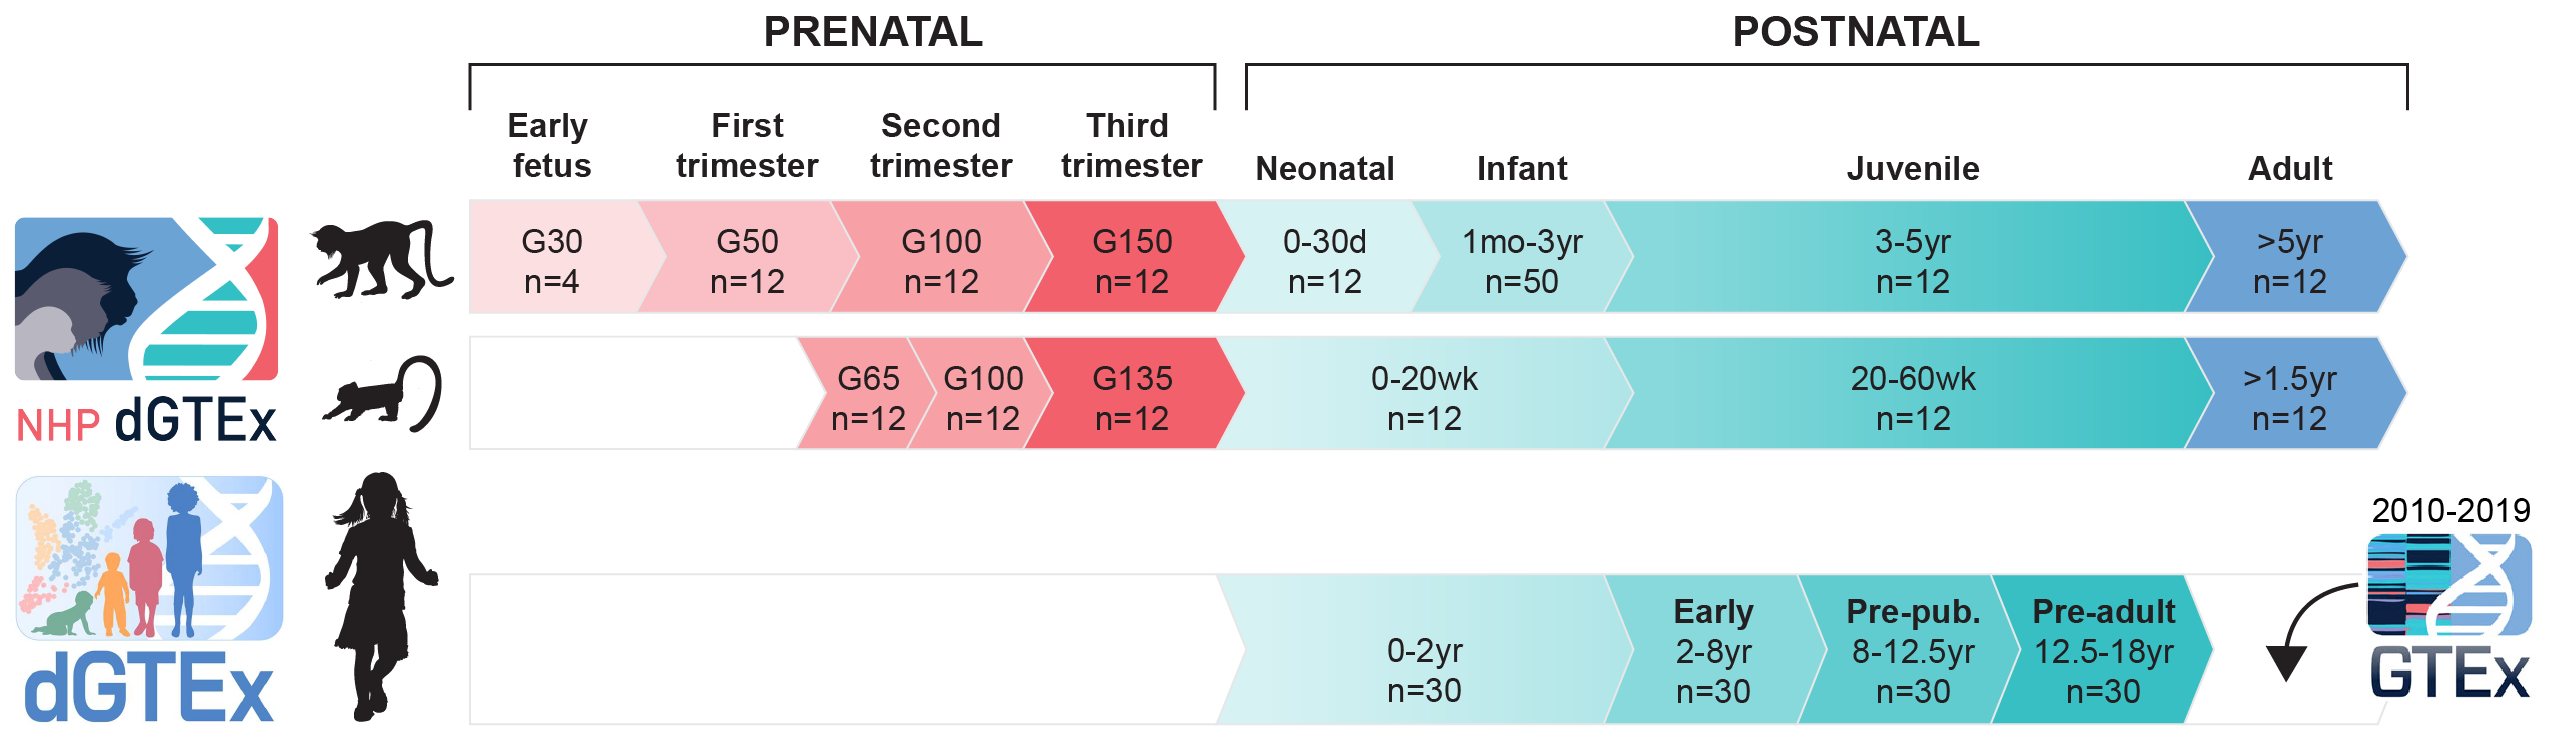
\includegraphics[width=0.95\textwidth]{cite_figures/attachment_dgtex_timeline_for_marker_paper}

    \vspace{0.5cm}
    \begin{center}
        {\cardiffLead{Comprehensive human developmental transcriptomics remains limited.}}\\[0.4em]
        {\tiny\color{CardiffDarkGrey}Coorens, T.H.H., Guillaumet-Adkins, A., Kovner, R. \textit{et al.} The human and non-human primate developmental GTEx projects. \textit{Nature} 637, 557--564 (2025). doi:10.1038/s41586-024-08244-9}
    \end{center}
\end{frame}

% ============================================================================
% SLIDE 3: The Challenge
% ============================================================================
\begin{frame}{The Challenge}
    \vspace{0.5cm}
    \begin{columns}[T, onlytextwidth]
        \column{0.48\textwidth}
            \hspace{0.22cm}\cardiffHeading{Current Gaps}
            \vspace{0.5em}
            \begin{itemize}
                \item No molecular standard to stage pigs; chronological age is unreliable.
                \item Tissue signals differ, so cross-tissue staging is inconsistent.
                \item Pig--human alignment is unclear; shared biomarkers are underused.
            \end{itemize}

        \column{0.48\textwidth}
            \cardiffHeading{Our Goal}
            \vspace{0.5em}
            \begin{itemize}
                \item \textbf{Gene Expression $\rightarrow$ Pig Age}: Define molecular developmental stages from transcriptomics.
                \item \textbf{Pig Age $\rightarrow$ Human Age}: Align pig stages to human timeline via conserved biomarkers.
                \item \textbf{Result}: A unified, cross-species molecular clock.
            \end{itemize}
    \end{columns}
\end{frame}

% ============================================================================
% SLIDE 3: Data Overview
% ============================================================================
\section{Data Overview}

\begin{frame}{The PigGTEx Project}
    \vspace{0.2cm}
    \begin{columns}[T, onlytextwidth]
        \column{0.52\textwidth}
            \hspace{0.22cm}\cardiffHeading{Context \& Mission}
            \vspace{0.3em}
            \begin{itemize}
                \item Part of the \textbf{FarmGTEx} consortium (Farm Animal Genotype-Tissue Expression).
                \item \textbf{Goal:} Build a comprehensive catalogue of genetic regulatory variants in pigs.
                \item Analyze \textbf{transcriptomic landscape} across diverse tissues and biological contexts.
            \end{itemize}

        \column{0.44\textwidth}
            \cardiffHeading{Key Objectives}
            \vspace{0.3em}
            \begin{itemize}
                \item \textbf{Genetic Mechanisms:} Link genetic variation to gene expression.
                \item \textbf{Biomedical Model:} Leverage pigs as models for human physiology and disease.
                \item \textbf{Sustainable Agriculture:} Inform breeding for health and efficiency.
            \end{itemize}
    \end{columns}
    
    \vspace{0.2cm}
    \begin{center}
        {\footnotesize\color{CardiffDarkGrey}
        \textbf{A massive public resource:} Integrating thousands of RNA-seq samples to map the pig regulatory genome.}
    \end{center}
\end{frame}

% ============================================================================
% SLIDE 3b: Data Quality Challenges
% ============================================================================
\begin{frame}{Data Quality Challenges}
    \vspace{0.3cm}
    \begin{columns}[T, onlytextwidth]
        \column{0.48\textwidth}
            \hspace{0.22cm}\cardiffHeading{Missing Data}
            \vspace{0.5em}
            \begin{itemize}
                \item \textbf{52\%} of samples missing age information
                \item \textbf{52\%} of samples missing sex labels
                \item \textbf{13\%} of samples with unknown tissue category
            \end{itemize}

        \column{0.48\textwidth}
            \cardiffHeading{Age Format Inconsistencies}
            \vspace{0.5em}
            {\small Age stored as text in various formats:}
            \vspace{0.3em}
            \begin{itemize}
                \item ``0 day'', ``1 day'', ``7 days''
                \item ``1 week'', ``2 weeks'', ``4 weeks''
                \item ``1 month'', ``3 months'', ``6 months''
                \item ``1 year'', ``2 years''
                \item ``unknown''
            \end{itemize}
            
            \vspace{0.3em}
            \begin{center}
                \color{CardiffRed}\textbf{Challenge:}\\
                \small Harmonize to a unified numeric format
            \end{center}
    \end{columns}
\end{frame}

% ============================================================================
% SLIDE 3c: Data Processing Pipeline
% ============================================================================
\begin{frame}{Data Processing Pipeline}
    \vspace{0.2cm}
    \begin{columns}[T, onlytextwidth]
        \column{0.48\textwidth}
            \hspace{0.22cm}\cardiffHeading{1. Age Harmonization}
            \vspace{0.3em}
            {\small
            \begin{itemize}
                \item Parse text $\rightarrow$ days
                \item Map to 5 biological stages:
            \end{itemize}
            \vspace{0.2em}
            \begin{center}
            \begin{tabular}{ll}
                \scriptsize Infant & \scriptsize 0--20 days \\
                \scriptsize Early childhood & \scriptsize 21--59 days \\
                \scriptsize Pre-pubertal & \scriptsize 60--149 days \\
                \scriptsize Post-pubertal & \scriptsize 150--365 days \\
                \scriptsize Adult & \scriptsize $>$365 days \\
            \end{tabular}
            \end{center}
            }
            
            \vspace{0.3em}
            \cardiffHeading{2. Expression Preprocessing}
            \vspace{0.3em}
            {\small
            \begin{itemize}
                \item Log$_2$(TPM + 1) transformation
            \end{itemize}
            }

        \column{0.48\textwidth}
            \cardiffHeading{3. Quality Control}
            \vspace{0.3em}
            {\small
            \begin{itemize}
                \item Filter samples with missing stage
                \item Explicit ``Unknown'' sex encoding
            \end{itemize}
            }
            
            \vspace{0.1em}
            \cardiffHeading{4. Adaptive Classification}
            \vspace{0.1em}
            {\small
            
            \textbf{4-class}:\\[-0.3em]
            \hspace{0.5em}Muscle, Liver\\[0.2em]
            \textbf{2-class}:\\[-0.3em]
            \hspace{0.5em}Lung, Blood, Brain\\[0.3em]
            \scriptsize\color{CardiffDarkGrey}\textit{Tissue-specific schemes ensure sufficient samples per class for ML training.}
            }
            
            \vspace{0.1em}
            \begin{center}
                \color{CardiffRed}$\downarrow$\\
                \textbf{2,467 curated samples}\\
                \small across 8 major tissues
            \end{center}
    \end{columns}
\end{frame}

\begin{frame}{Classification Schemes}
    \centering
    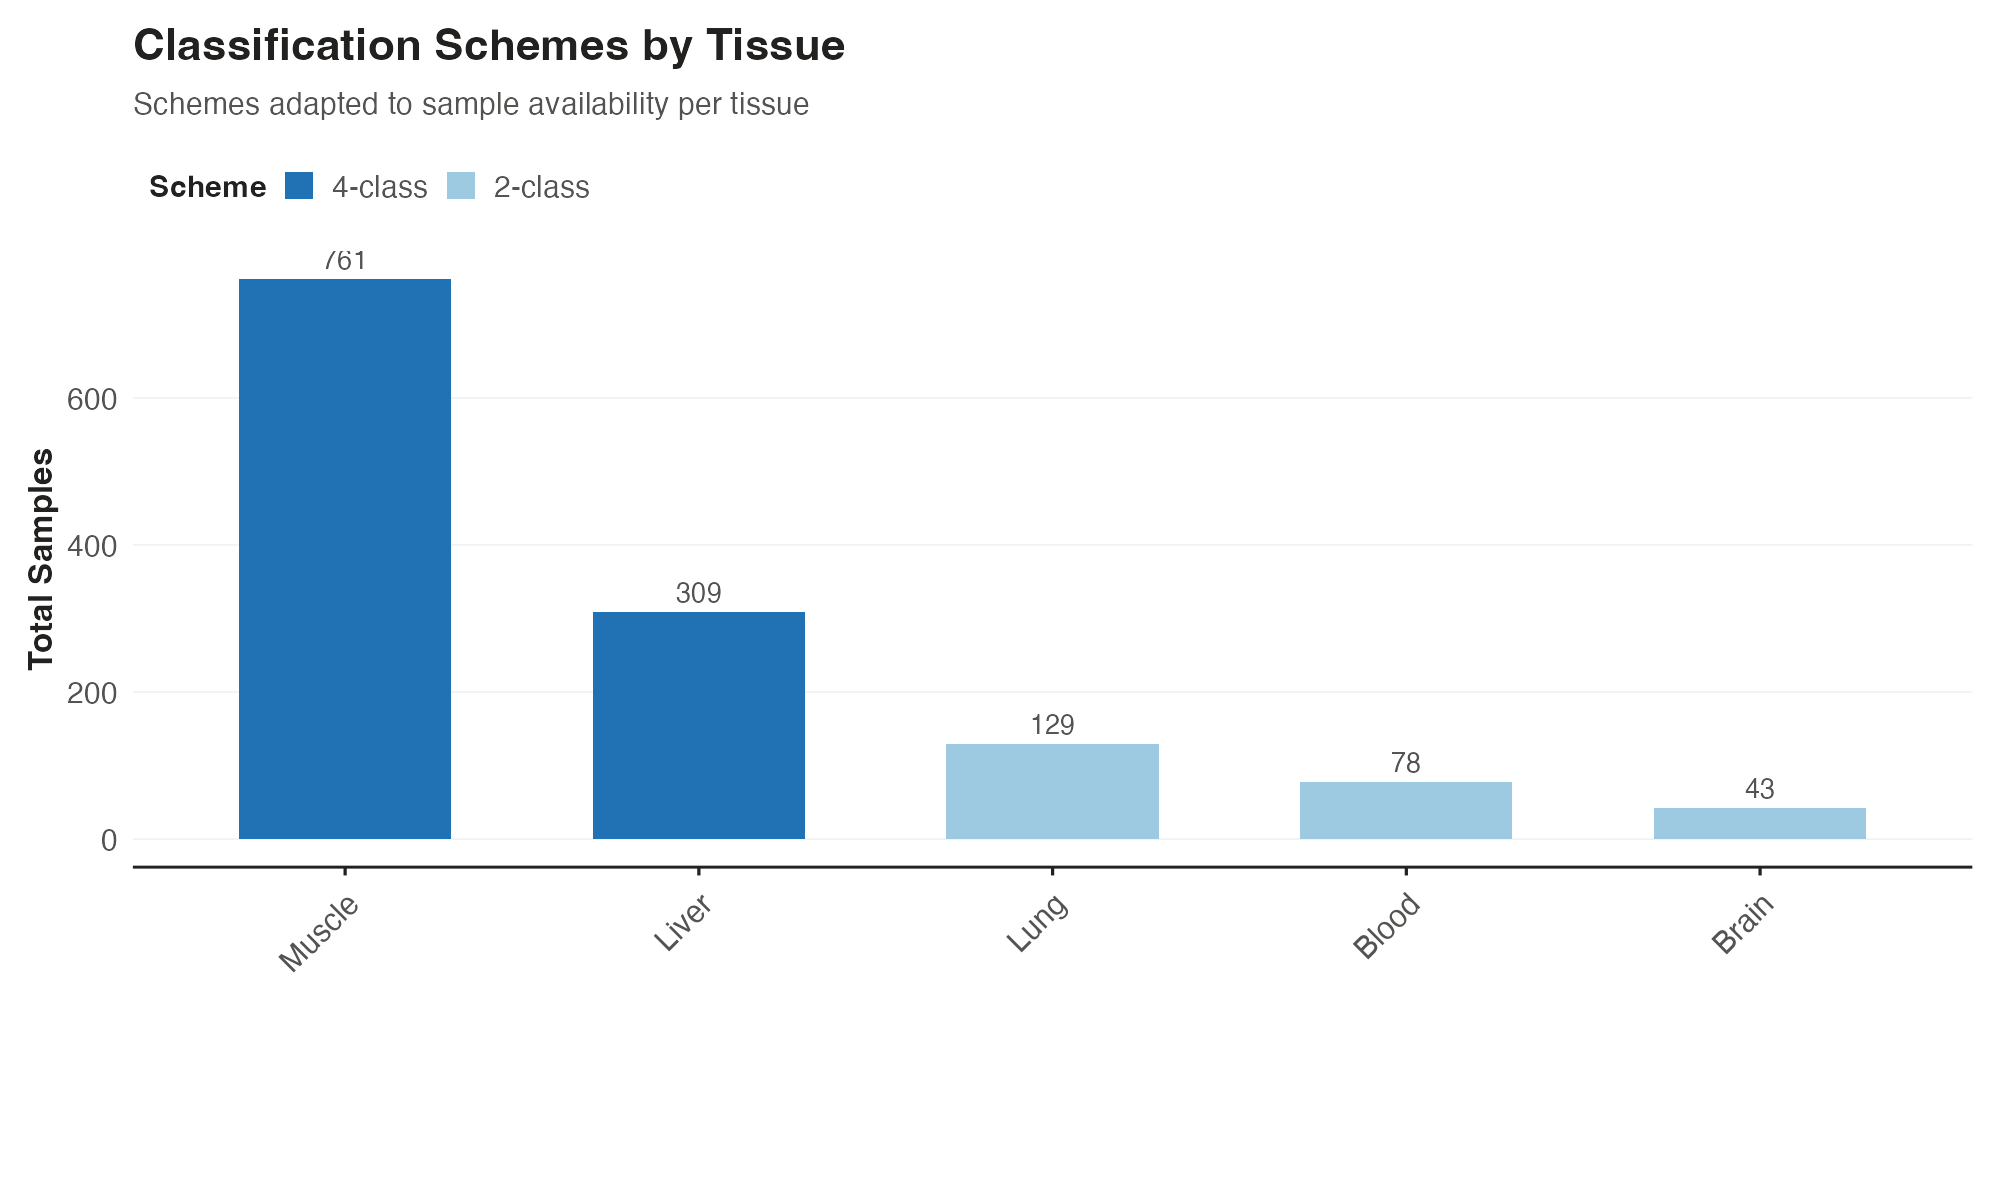
\includegraphics[width=0.85\textwidth]{Figures/fig1_panel_b_classification_schemes}
\end{frame}

\begin{frame}{Dataset: pigGTEx}
    \vspace{0.5cm}
    \begin{columns}[T]
        \column{0.35\textwidth}
            \textbf{Scale \& Scope}
            \vspace{0.5em}
            \begin{itemize}
                \item \textbf{2,467 samples} across \textbf{8 tissues/cell types}.
                \item Comprehensive sequencing of:
                \begin{itemize}
                    \item Muscle, Brain, Liver, Blood
                    \item Intestine, Lung, Adipose, Testis
                \end{itemize}
            \end{itemize}

        \column{0.6\textwidth}
            \centering
            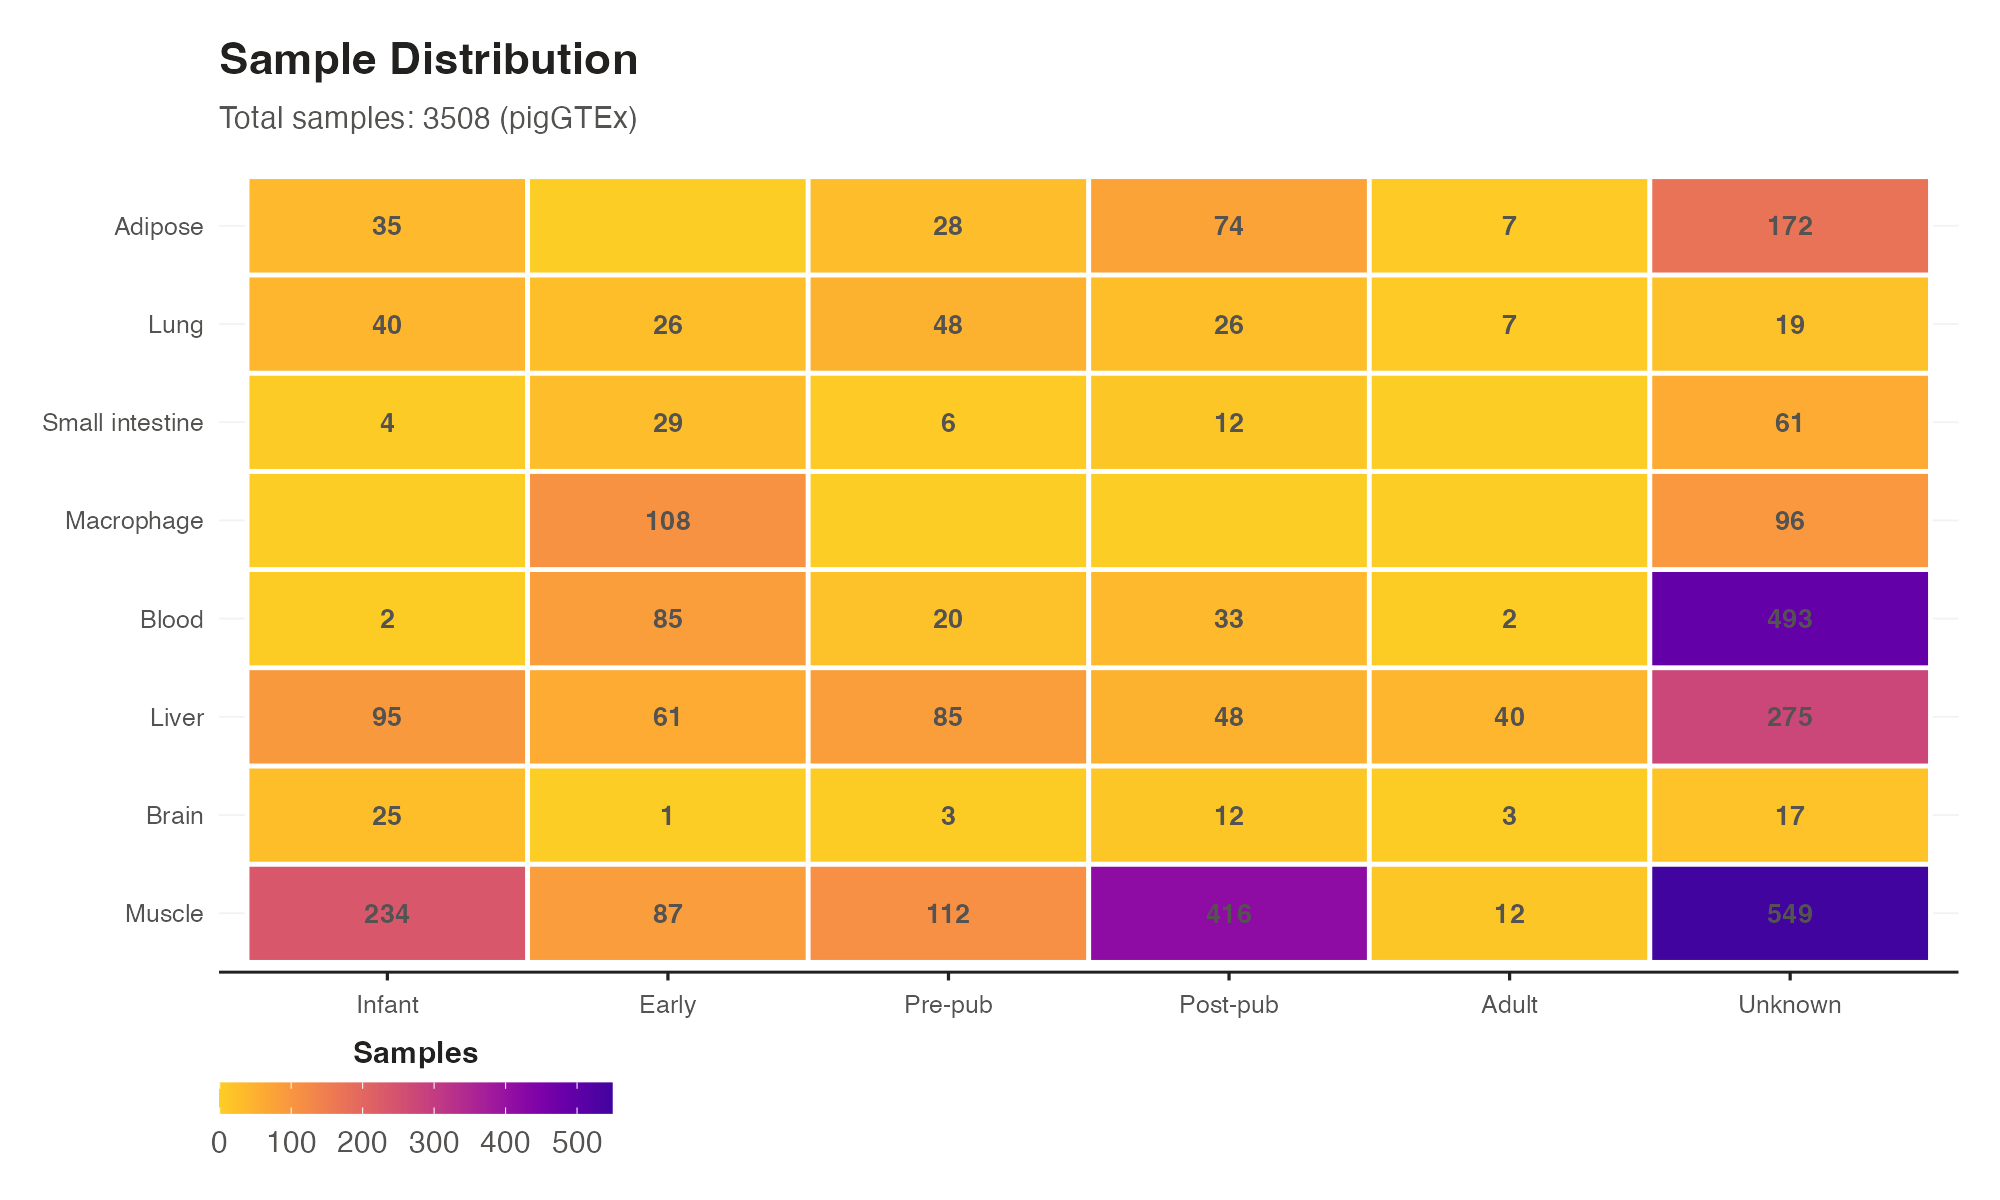
\includegraphics[width=\textwidth]{Figures/fig1_panel_a_sample_distribution}
    \end{columns}
\end{frame}

% ============================================================================
% SLIDE 4: Methodology
% ============================================================================
\section{Methodology}

% Methodology overview (compact TOC)
\begin{frame}{Methodology Overview}
    \vspace{0.2cm}
    \begin{columns}[T]
        \column{0.32\textwidth}
            \textbf{1. Classification}
            \vspace{0.25em}
            {\small
            \begin{itemize}
                \item Multi-resolution schemes
                \item 4-class / 3-class / Binary
            \end{itemize}}
            
        \column{0.32\textwidth}
            \textbf{2. Machine Learning}
            \vspace{0.25em}
            {\small
            \begin{itemize}
                \item Ordinal LightGBM
                \item Binary reduction strategy
            \end{itemize}}
            
        \column{0.32\textwidth}
            \textbf{3. Validation}
            \vspace{0.25em}
            {\small
            \begin{itemize}
                \item Tissue-specific performance
                \item Cross-tissue robustness
            \end{itemize}}
    \end{columns}
\end{frame}



% ============================================================================
% SLIDE 4b: The Machine Learning Problem (X and Y)
% ============================================================================
\begin{frame}{The Machine Learning Problem}
    \vspace{0.1cm}
    \begin{columns}[T, onlytextwidth]
        \column{0.48\textwidth}
            \hspace{0.22cm}\cardiffHeading{What is X? (Features)}
            \vspace{0.3em}
            {\small \textbf{Gene expression values} from RNA-seq}
            \vspace{0.2em}
            \begin{center}
            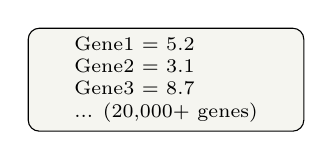
\begin{tikzpicture}[scale=0.65]
                \node[draw, rounded corners, fill=CardiffSuperLightGrey, minimum width=3.5cm, align=left, font=\scriptsize] at (0,0) {
                    Gene1 = 5.2\\
                    Gene2 = 3.1\\
                    Gene3 = 8.7\\
                    ... (20,000+ genes)
                };
            \end{tikzpicture}
            \end{center}
            {\scriptsize Each sample = one pig's gene expression profile}

        \column{0.48\textwidth}
            \cardiffHeading{What is Y? (Label)}
            \vspace{0.3em}
            {\small \textbf{Developmental stage} we want to predict}
            \vspace{0.2em}
            \begin{center}
            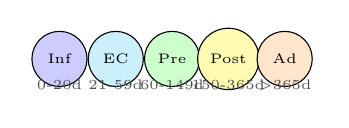
\begin{tikzpicture}[scale=0.55]
                \node[draw, circle, fill=blue!20, minimum size=0.7cm, font=\tiny] (i) at (0,0) {Inf};
                \node[draw, circle, fill=cyan!20, minimum size=0.7cm, font=\tiny] (ec) at (1.3,0) {EC};
                \node[draw, circle, fill=green!20, minimum size=0.7cm, font=\tiny] (pre) at (2.6,0) {Pre};
                \node[draw, circle, fill=yellow!30, minimum size=0.7cm, font=\tiny] (post) at (3.9,0) {Post};
                \node[draw, circle, fill=orange!20, minimum size=0.7cm, font=\tiny] (a) at (5.2,0) {Ad};
                \node[font=\tiny, color=CardiffDarkGrey] at (0,-0.6) {0-20d};
                \node[font=\tiny, color=CardiffDarkGrey] at (1.3,-0.6) {21-59d};
                \node[font=\tiny, color=CardiffDarkGrey] at (2.6,-0.6) {60-149d};
                \node[font=\tiny, color=CardiffDarkGrey] at (3.9,-0.6) {150-365d};
                \node[font=\tiny, color=CardiffDarkGrey] at (5.2,-0.6) {$>$365d};
            \end{tikzpicture}
            \end{center}
            {\scriptsize Goal: Gene expression $\rightarrow$ Predict stage}
    \end{columns}
    
    \vspace{0.3cm}
    \begin{center}
        \fcolorbox{CardiffRed}{CardiffSuperLightGrey}{\parbox{0.75\textwidth}{\centering
            \small\textbf{In simple terms:} Given a pig's gene activity, which developmental stage is it in?
        }}
    \end{center}
\end{frame}

% ============================================================================
% SLIDE 4c: Why Machine Learning?
% ============================================================================
\begin{frame}{Why Machine Learning?}
    \vspace{0.3cm}
    \begin{columns}[t, onlytextwidth]
        \column{0.32\textwidth}
            \centering
            \hspace{0.22cm}\cardiffHeading{Traditional Regression}
            \vspace{0.5em}
            
            % Fixed height box for diagram
            \begin{minipage}[t][2.2cm][c]{\linewidth}
                \centering
                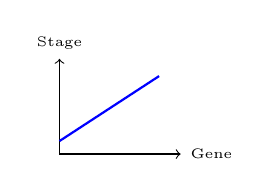
\begin{tikzpicture}[scale=0.55]
                    \draw[->] (0,0) -- (2.8,0) node[right, font=\tiny] {Gene};
                    \draw[->] (0,0) -- (0,2.2) node[above, font=\tiny] {Stage};
                    \draw[thick, blue] (0,0.3) -- (2.3,1.8);
                \end{tikzpicture}
            \end{minipage}
            
            \vspace{0.3em}
            {\scriptsize
            \begin{itemize}\setlength{\itemsep}{2pt}
                \item Assumes linear relationships
                \item \textcolor{red}{Genes interact non-linearly!}
            \end{itemize}}

        \column{0.32\textwidth}
            \centering
            \cardiffHeading{Deep Learning}
            \vspace{0.5em}
            
            % Fixed height box for diagram
            \begin{minipage}[t][2.2cm][c]{\linewidth}
                \centering
                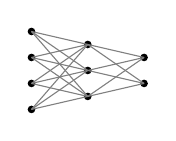
\begin{tikzpicture}[scale=0.55]
                    \foreach \y in {0.3,0.9,1.5,2.1} \fill (0,\y) circle (2.5pt);
                    \foreach \y in {0.6,1.2,1.8} \fill (1.3,\y) circle (2.5pt);
                    \foreach \y in {0.9,1.5} \fill (2.6,\y) circle (2.5pt);
                    \foreach \a in {0.3,0.9,1.5,2.1} \foreach \b in {0.6,1.2,1.8} \draw[gray, thin] (0,\a) -- (1.3,\b);
                    \foreach \a in {0.6,1.2,1.8} \foreach \b in {0.9,1.5} \draw[gray, thin] (1.3,\a) -- (2.6,\b);
                \end{tikzpicture}
            \end{minipage}
            
            \vspace{0.3em}
            {\scriptsize
            \begin{itemize}\setlength{\itemsep}{2pt}
                \item Needs \textbf{thousands} of samples
                \item \textcolor{red}{We only have hundreds!}
            \end{itemize}}

        \column{0.32\textwidth}
            \centering
            \cardiffHeading{LightGBM \checkmark}
            \vspace{0.5em}
            
            % Fixed height box for diagram
            \begin{minipage}[t][2.2cm][c]{\linewidth}
                \centering
                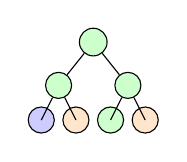
\begin{tikzpicture}[scale=0.55]
                    \node[draw, circle, fill=green!20, minimum size=10pt] (root) at (1.2,2) {};
                    \node[draw, circle, fill=green!20, minimum size=8pt] (l) at (0.4,1) {};
                    \node[draw, circle, fill=green!20, minimum size=8pt] (r) at (2,1) {};
                    \node[draw, circle, fill=blue!20, minimum size=7pt] at (0,0.2) {};
                    \node[draw, circle, fill=orange!20, minimum size=7pt] at (0.8,0.2) {};
                    \node[draw, circle, fill=green!20, minimum size=7pt] at (1.6,0.2) {};
                    \node[draw, circle, fill=orange!20, minimum size=7pt] at (2.4,0.2) {};
                    \draw (root) -- (l); \draw (root) -- (r);
                    \draw (l) -- (0,0.2); \draw (l) -- (0.8,0.2);
                    \draw (r) -- (1.6,0.2); \draw (r) -- (2.4,0.2);
                \end{tikzpicture}
            \end{minipage}
            
            \vspace{0.3em}
            {\scriptsize
            \begin{itemize}\setlength{\itemsep}{2pt}
                \item Handles \textbf{non-linear} patterns
                \item Works with \textbf{small samples}
            \end{itemize}}
    \end{columns}
    
    \vspace{0.4cm}
    \begin{center}
        \color{CardiffRed}\textbf{LightGBM: Best performance with limited sample sizes}
    \end{center}
\end{frame}

% ============================================================================
% SLIDE 4d: How Does a Decision Tree Work?
% ============================================================================
\begin{frame}{How Does a Decision Tree Work?}
    \vspace{0.1cm}
    \cardiffHeading{Simple Example: 3 Genes to Predict Stage}
    \vspace{0.2cm}
    
    \begin{columns}[T]
        \column{0.55\textwidth}
            \begin{center}
            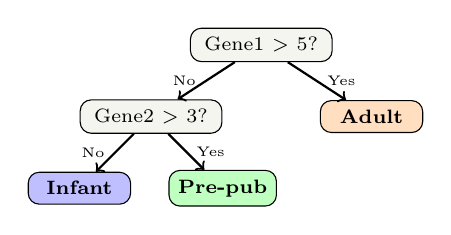
\begin{tikzpicture}[scale=0.7, 
                every node/.style={font=\scriptsize},
                decision/.style={draw, rounded corners, fill=CardiffSuperLightGrey, minimum width=1.8cm, align=center},
                leaf/.style={draw, rounded corners, minimum width=1.3cm, align=center}]
                
                % Root
                \node[decision] (root) at (0,0) {Gene1 $>$ 5?};
                
                % Level 1
                \node[decision] (l1) at (-2,-1.3) {Gene2 $>$ 3?};
                \node[leaf, fill=orange!25] (r1) at (2,-1.3) {\textbf{Adult}};
                
                % Level 2
                \node[leaf, fill=blue!25] (ll) at (-3.3,-2.6) {\textbf{Infant}};
                \node[leaf, fill=green!25] (lr) at (-0.7,-2.6) {\textbf{Pre-pub}};
                
                % Edges
                \draw[->, thick] (root) -- node[left, font=\tiny] {No} (l1);
                \draw[->, thick] (root) -- node[right, font=\tiny] {Yes} (r1);
                \draw[->, thick] (l1) -- node[left, font=\tiny] {No} (ll);
                \draw[->, thick] (l1) -- node[right, font=\tiny] {Yes} (lr);
            \end{tikzpicture}
            \end{center}

        \column{0.42\textwidth}
            \cardiffHeading{How it works:}
            \vspace{0.2em}
            {\small
            \begin{enumerate}\setlength{\itemsep}{0pt}
                \item Start at the top
                \item Ask yes/no questions about genes
                \item Follow branches to decision
            \end{enumerate}}
            
            \vspace{0.3em}
            {\small\textbf{Example:} Gene1=6.2, Gene2=2.1}
            \vspace{0.2em}
            {\small
            \begin{itemize}\setlength{\itemsep}{0pt}
                \item Gene1 $>$ 5? \textcolor{green!50!black}{\textbf{Yes}} $\rightarrow$ \textbf{Adult ($>$365d)}
            \end{itemize}}
    \end{columns}
    
    \vspace{0.2cm}
    \begin{center}
        \color{CardiffDarkGrey}\scriptsize
        A single tree asks simple questions about genes to classify developmental stage.
    \end{center}
\end{frame}

% ============================================================================
% SLIDE 4e: From One Tree to Many Trees
% ============================================================================
\begin{frame}{From One Tree to Many Trees}
    \vspace{0.2cm}
    \cardiffHeading{One tree can make mistakes. Many trees vote together!}
    \vspace{0.4cm}
    
    \begin{columns}[T]
        \column{0.55\textwidth}
            \begin{center}
            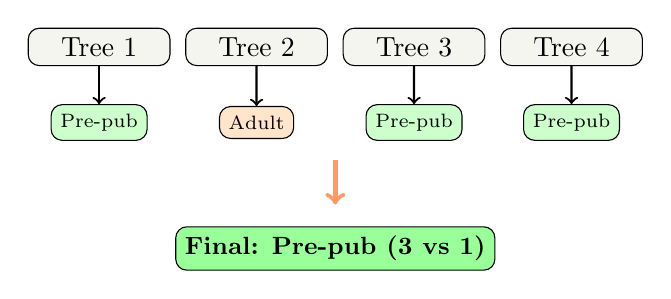
\begin{tikzpicture}[scale=0.8]
                % Trees
                \node[draw, rounded corners, fill=CardiffSuperLightGrey, minimum width=1.8cm] (t1) at (0,2) {Tree 1};
                \node[draw, rounded corners, fill=CardiffSuperLightGrey, minimum width=1.8cm] (t2) at (2.5,2) {Tree 2};
                \node[draw, rounded corners, fill=CardiffSuperLightGrey, minimum width=1.8cm] (t3) at (5,2) {Tree 3};
                \node[draw, rounded corners, fill=CardiffSuperLightGrey, minimum width=1.8cm] (t4) at (7.5,2) {Tree 4};
                
                % Predictions
                \node[draw, rounded corners, fill=green!20, font=\scriptsize] (p1) at (0,0.8) {Pre-pub};
                \node[draw, rounded corners, fill=orange!20, font=\scriptsize] (p2) at (2.5,0.8) {Adult};
                \node[draw, rounded corners, fill=green!20, font=\scriptsize] (p3) at (5,0.8) {Pre-pub};
                \node[draw, rounded corners, fill=green!20, font=\scriptsize] (p4) at (7.5,0.8) {Pre-pub};
                
                \draw[->, thick] (t1) -- (p1);
                \draw[->, thick] (t2) -- (p2);
                \draw[->, thick] (t3) -- (p3);
                \draw[->, thick] (t4) -- (p4);
                
                % Vote arrow
                \draw[->, ultra thick, CardiffRed] (3.75,0.2) -- (3.75,-0.5);
                
                % Final result
                \node[draw, rounded corners, fill=green!40, font=\small\bfseries, minimum width=3cm] at (3.75,-1.2) {Final: Pre-pub (3 vs 1)};
            \end{tikzpicture}
            \end{center}

        \column{0.42\textwidth}
            \cardiffHeading{Why multiple trees?}
            \vspace{0.3em}
            \begin{itemize}
                \item Each tree sees data differently
                \item Mistakes cancel out
                \item \textbf{Majority vote} is more reliable
            \end{itemize}
            
            \vspace{0.5em}
            \fcolorbox{CardiffRed}{CardiffSuperLightGrey}{\parbox{0.9\linewidth}{\centering
                \small More trees = More reliable predictions!
            }}
    \end{columns}
\end{frame}

% ============================================================================
% SLIDE 4f: What Makes LightGBM Special - Boosting
% ============================================================================
\begin{frame}{What Makes LightGBM Special: Boosting}
    \vspace{0.1cm}
    \cardiffHeading{Each new tree learns from previous mistakes}
    \vspace{0.2cm}
    
    \begin{center}
    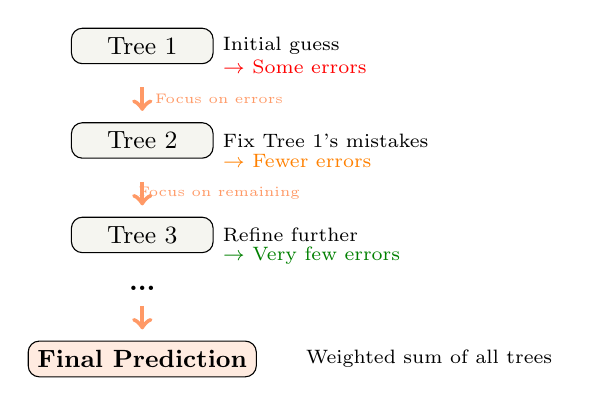
\begin{tikzpicture}[scale=0.75]
        % Tree 1
        \node[draw, rounded corners, fill=CardiffSuperLightGrey, minimum width=1.8cm, font=\small] (t1) at (0,0) {Tree 1};
        \node[font=\scriptsize, anchor=west] at (1.2,0) {Initial guess};
        \node[font=\scriptsize, color=red, anchor=west] at (1.2,-0.35) {$\rightarrow$ Some errors};
        
        % Arrow
        \draw[->, ultra thick, CardiffRed] (0,-0.7) -- (0,-1.1);
        \node[font=\tiny, color=CardiffRed] at (1.3,-0.9) {Focus on errors};
        
        % Tree 2
        \node[draw, rounded corners, fill=CardiffSuperLightGrey, minimum width=1.8cm, font=\small] (t2) at (0,-1.6) {Tree 2};
        \node[font=\scriptsize, anchor=west] at (1.2,-1.6) {Fix Tree 1's mistakes};
        \node[font=\scriptsize, color=orange, anchor=west] at (1.2,-1.95) {$\rightarrow$ Fewer errors};
        
        % Arrow
        \draw[->, ultra thick, CardiffRed] (0,-2.3) -- (0,-2.7);
        \node[font=\tiny, color=CardiffRed] at (1.3,-2.5) {Focus on remaining};
        
        % Tree 3
        \node[draw, rounded corners, fill=CardiffSuperLightGrey, minimum width=1.8cm, font=\small] (t3) at (0,-3.2) {Tree 3};
        \node[font=\scriptsize, anchor=west] at (1.2,-3.2) {Refine further};
        \node[font=\scriptsize, color=green!50!black, anchor=west] at (1.2,-3.55) {$\rightarrow$ Very few errors};
        
        % Dots and final
        \node at (0,-4.1) {\textbf{...}};
        \draw[->, ultra thick, CardiffRed] (0,-4.4) -- (0,-4.8);
        \node[draw, rounded corners, fill=CardiffRed!20, minimum width=2.2cm, font=\small\bfseries] (final) at (0,-5.3) {Final Prediction};
        \node[font=\scriptsize, anchor=west, xshift=0.5cm] at (final.east) {Weighted sum of all trees};
    \end{tikzpicture}
    \end{center}
    
    \vspace{0.1cm}
    \begin{center}
        \fcolorbox{CardiffRed}{CardiffSuperLightGrey}{\parbox{0.65\textwidth}{\centering
            \small\textbf{Boosting:} Trees work as a team, each fixing the others' mistakes
        }}
    \end{center}
\end{frame}

% ============================================================================
% SLIDE 4g: Why Ordinal Classification?
% ============================================================================
\begin{frame}{Why Ordinal Classification Matters}
    \vspace{0.3cm}
    \begin{columns}[T, onlytextwidth]
        \column{0.5\textwidth}
            \hspace{0.22cm}\cardiffHeading{Developmental Stages Have Order}
            \vspace{0.5em}
            
            \begin{center}
            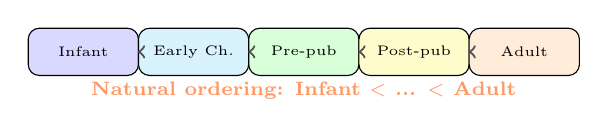
\begin{tikzpicture}[scale=0.7]
                % Stage boxes with gradient colors - 5 stages
                \node[draw, rounded corners, fill=blue!15, minimum width=1.4cm, minimum height=0.6cm, font=\tiny] (i) at (0,0) {Infant};
                \node[draw, rounded corners, fill=cyan!15, minimum width=1.4cm, minimum height=0.6cm, font=\tiny] (ec) at (2,0) {Early Ch.};
                \node[draw, rounded corners, fill=green!15, minimum width=1.4cm, minimum height=0.6cm, font=\tiny] (pre) at (4,0) {Pre-pub};
                \node[draw, rounded corners, fill=yellow!20, minimum width=1.4cm, minimum height=0.6cm, font=\tiny] (post) at (6,0) {Post-pub};
                \node[draw, rounded corners, fill=orange!15, minimum width=1.4cm, minimum height=0.6cm, font=\tiny] (a) at (8,0) {Adult};
                
                % Arrows showing order
                \draw[->, thick, CardiffDarkGrey] (i) -- (ec);
                \draw[->, thick, CardiffDarkGrey] (ec) -- (pre);
                \draw[->, thick, CardiffDarkGrey] (pre) -- (post);
                \draw[->, thick, CardiffDarkGrey] (post) -- (a);
                
                % Order label
                \node[font=\scriptsize, color=CardiffRed] at (4,-0.7) {\textbf{Natural ordering: Infant $<$ ... $<$ Adult}};
            \end{tikzpicture}
            \end{center}
            
            \vspace{0.3em}
            \textbf{\color{CardiffRed} Key insight:}\\
            Misclassifying Adult as Infant is \textbf{worse} than as Post-pubertal!

        \column{0.48\textwidth}
            \cardiffHeading{Standard vs Ordinal Approach}
            \vspace{0.8em}
            
            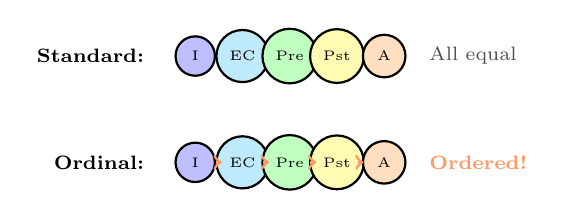
\begin{tikzpicture}[scale=0.75]
                % Standard classification - circles with clear spacing, no connection
                \node[font=\scriptsize\bfseries, anchor=east] at (0.5,2.8) {Standard:};
                \node[draw, circle, fill=blue!25, minimum size=0.5cm, font=\tiny, line width=0.8pt] (s1) at (1.2,2.8) {I};
                \node[draw, circle, fill=cyan!25, minimum size=0.5cm, font=\tiny, line width=0.8pt] (s2) at (2.0,2.8) {EC};
                \node[draw, circle, fill=green!25, minimum size=0.5cm, font=\tiny, line width=0.8pt] (s3) at (2.8,2.8) {Pre};
                \node[draw, circle, fill=yellow!30, minimum size=0.5cm, font=\tiny, line width=0.8pt] (s4) at (3.6,2.8) {Pst};
                \node[draw, circle, fill=orange!25, minimum size=0.5cm, font=\tiny, line width=0.8pt] (s5) at (4.4,2.8) {A};
                \node[font=\scriptsize, color=CardiffDarkGrey, anchor=west] at (5.0,2.8) {All equal};
                
                % Ordinal classification - connected with solid line and arrows
                \node[font=\scriptsize\bfseries, anchor=east] at (0.5,1.0) {Ordinal:};
                % Draw the connecting line FIRST (behind circles)
                \draw[-, thick, CardiffDarkGrey, line width=1.5pt] (1.2,1.0) -- (4.4,1.0);
                % Now draw circles on top of the line
                \node[draw, circle, fill=blue!25, minimum size=0.5cm, font=\tiny, line width=0.8pt] (o1) at (1.2,1.0) {I};
                \node[draw, circle, fill=cyan!25, minimum size=0.5cm, font=\tiny, line width=0.8pt] (o2) at (2.0,1.0) {EC};
                \node[draw, circle, fill=green!25, minimum size=0.5cm, font=\tiny, line width=0.8pt] (o3) at (2.8,1.0) {Pre};
                \node[draw, circle, fill=yellow!30, minimum size=0.5cm, font=\tiny, line width=0.8pt] (o4) at (3.6,1.0) {Pst};
                \node[draw, circle, fill=orange!25, minimum size=0.5cm, font=\tiny, line width=0.8pt] (o5) at (4.4,1.0) {A};
                % Add directional arrows between circles
                \draw[->, thick, CardiffRed, line width=1pt] (1.55,1.0) -- (1.65,1.0);
                \draw[->, thick, CardiffRed, line width=1pt] (2.35,1.0) -- (2.45,1.0);
                \draw[->, thick, CardiffRed, line width=1pt] (3.15,1.0) -- (3.25,1.0);
                \draw[->, thick, CardiffRed, line width=1pt] (3.95,1.0) -- (4.05,1.0);
                \node[font=\scriptsize, color=CardiffRed, anchor=west] at (5.0,1.0) {\textbf{Ordered!}};
            \end{tikzpicture}
            
            \vspace{0.5em}
            \textbf{Ordinal models:}
            \begin{itemize}
                \item Respect stage ordering
                \item Penalize distant errors more
                \item Better calibrated probabilities
            \end{itemize}
    \end{columns}
\end{frame}

% ============================================================================
% SLIDE 5: Results - Performance
% ============================================================================
\section{Results}

% Transition slide


\begin{frame}{Performance Metrics Overview}
    \vspace{0.3cm}
    \begin{columns}[T, onlytextwidth]
        \column{0.48\textwidth}
            \hspace{0.22cm}\cardiffHeading{Precision}
            \vspace{0.2em}
            {\small \color{CardiffDarkGrey} Proportion of positive identifications that were actually correct.}
            \begin{center}
                \fcolorbox{CardiffGrey}{CardiffSuperLightGrey}{%
                    $ \text{Precision} = \frac{TP}{TP + FP} $%
                }
            \end{center}
            
            \vspace{0.4em}
            \cardiffHeading{Recall}
            \vspace{0.2em}
            {\small \color{CardiffDarkGrey} Proportion of actual positives identified correctly.}
            \begin{center}
                \fcolorbox{CardiffGrey}{CardiffSuperLightGrey}{%
                    $ \text{Recall} = \frac{TP}{TP + FN} $%
                }
            \end{center}

        \column{0.48\textwidth}
            \cardiffHeading{F1 Score}
            \vspace{0.2em}
            {\small \color{CardiffDarkGrey} Harmonic mean of Precision \& Recall.}
            \begin{center}
                \fcolorbox{CardiffGrey}{CardiffSuperLightGrey}{%
                    $ \text{F1} = 2 \cdot \frac{\text{Precision} \cdot \text{Recall}}{\text{Precision} + \text{Recall}} $%
                }
            \end{center}
            
            \vspace{0.4em}
            \cardiffHeading{MCC (Matthews Correlation Coefficient)}
            \vspace{0.2em}
            {\small \color{CardiffDarkGrey} Balanced measure for imbalanced datasets.}
            \begin{center}
                \fcolorbox{CardiffGrey}{CardiffSuperLightGrey}{%
                    \resizebox{0.9\textwidth}{!}{%
                    $ \text{MCC} = \frac{TP \cdot TN - FP \cdot FN}{\sqrt{(TP+FP)(TP+FN)(TN+FP)(TN+FN)}} $%
                    }
                }
            \end{center}
    \end{columns}
\end{frame}

\begin{frame}{Model Performance}
    \centering
    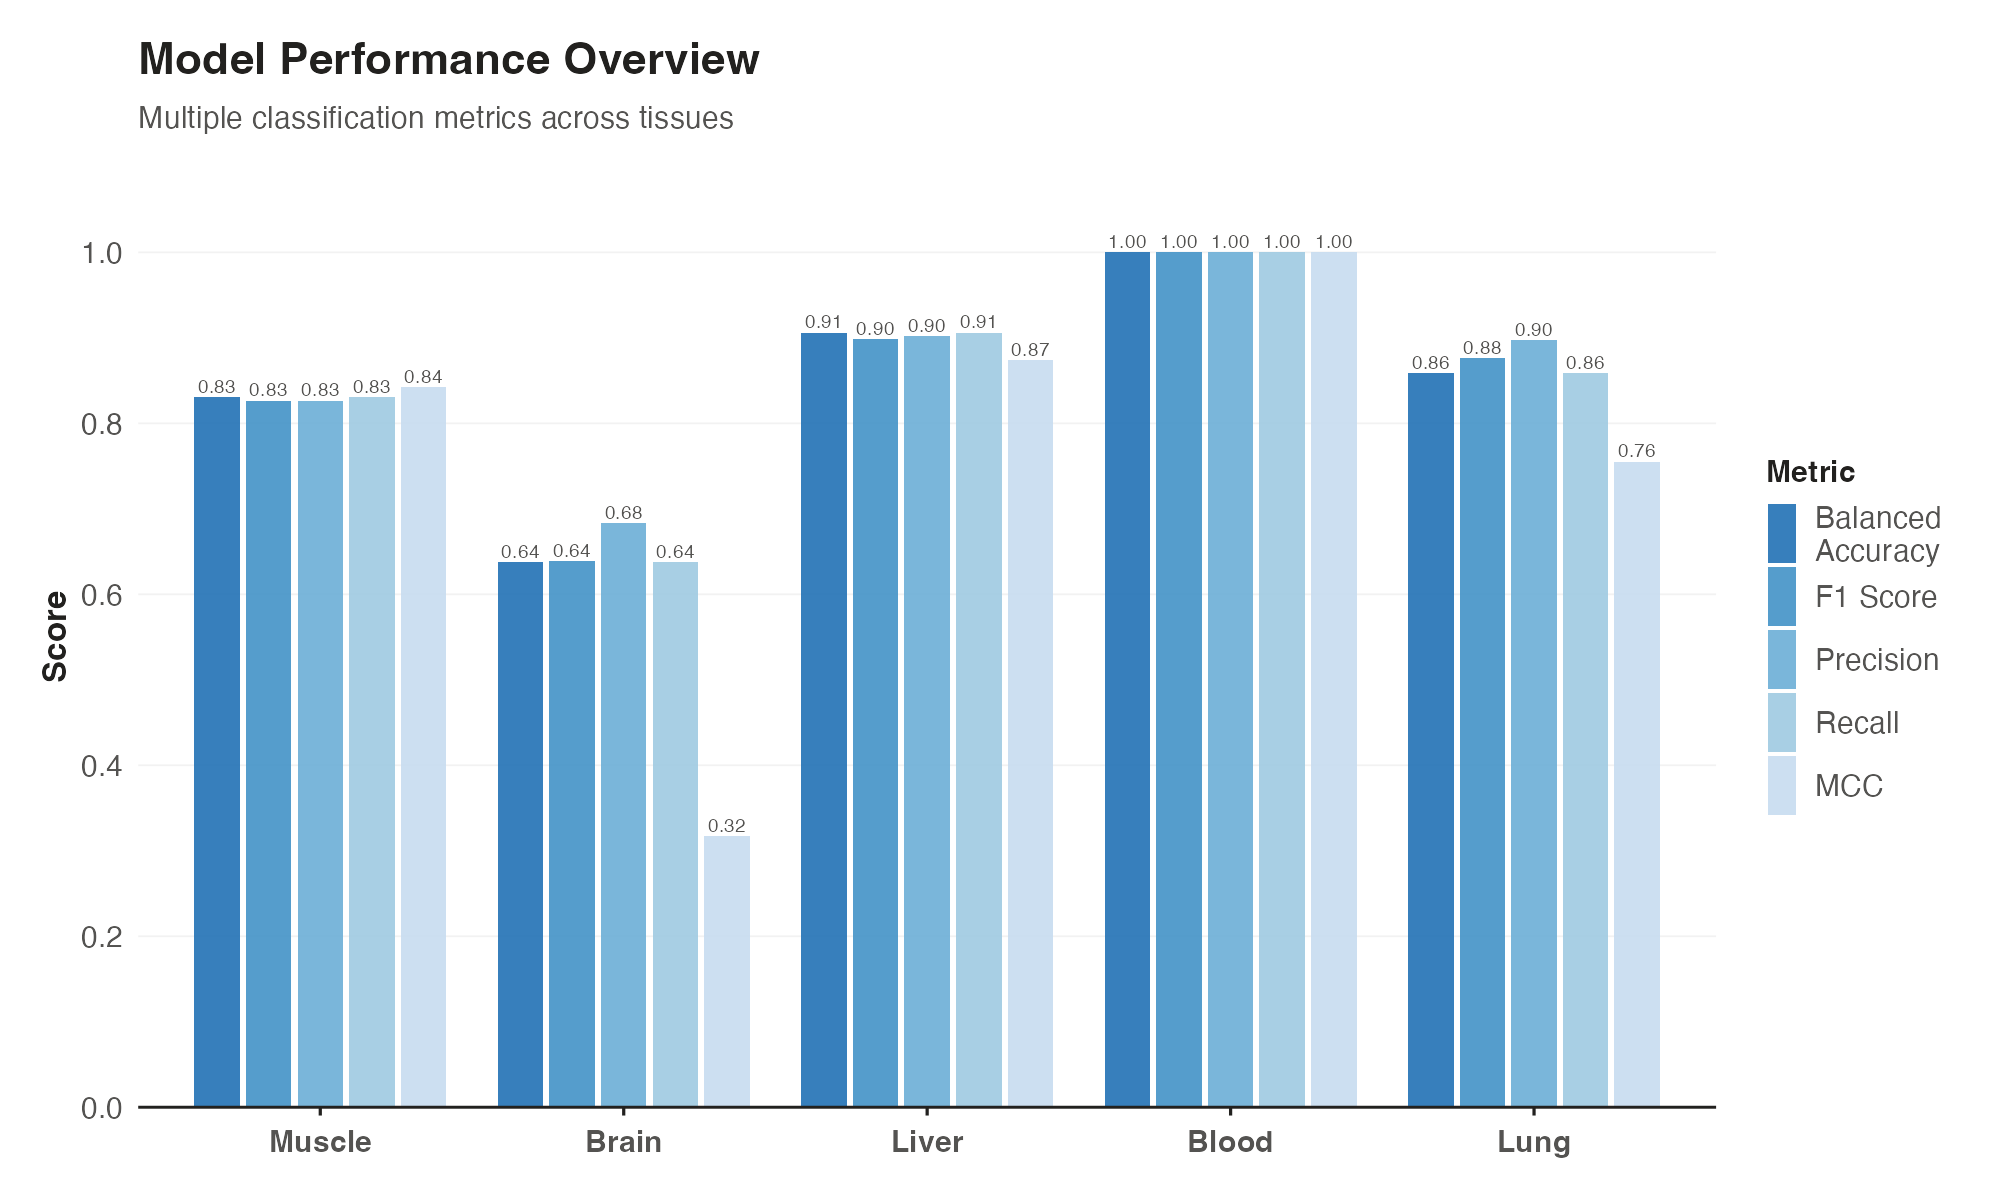
\includegraphics[width=0.85\textwidth, height=0.65\textheight, keepaspectratio]{Figures/fig2_panel_a_performance_metrics}
    
    \vspace{0.1cm}
    \begin{center}
        \textbf{\color{CardiffDarkGrey} Strong performance across all metrics: Balanced Accuracy, F1, Precision, Recall, MCC}
    \end{center}
\end{frame}

\begin{frame}{Confusion Matrices}
    \centering
    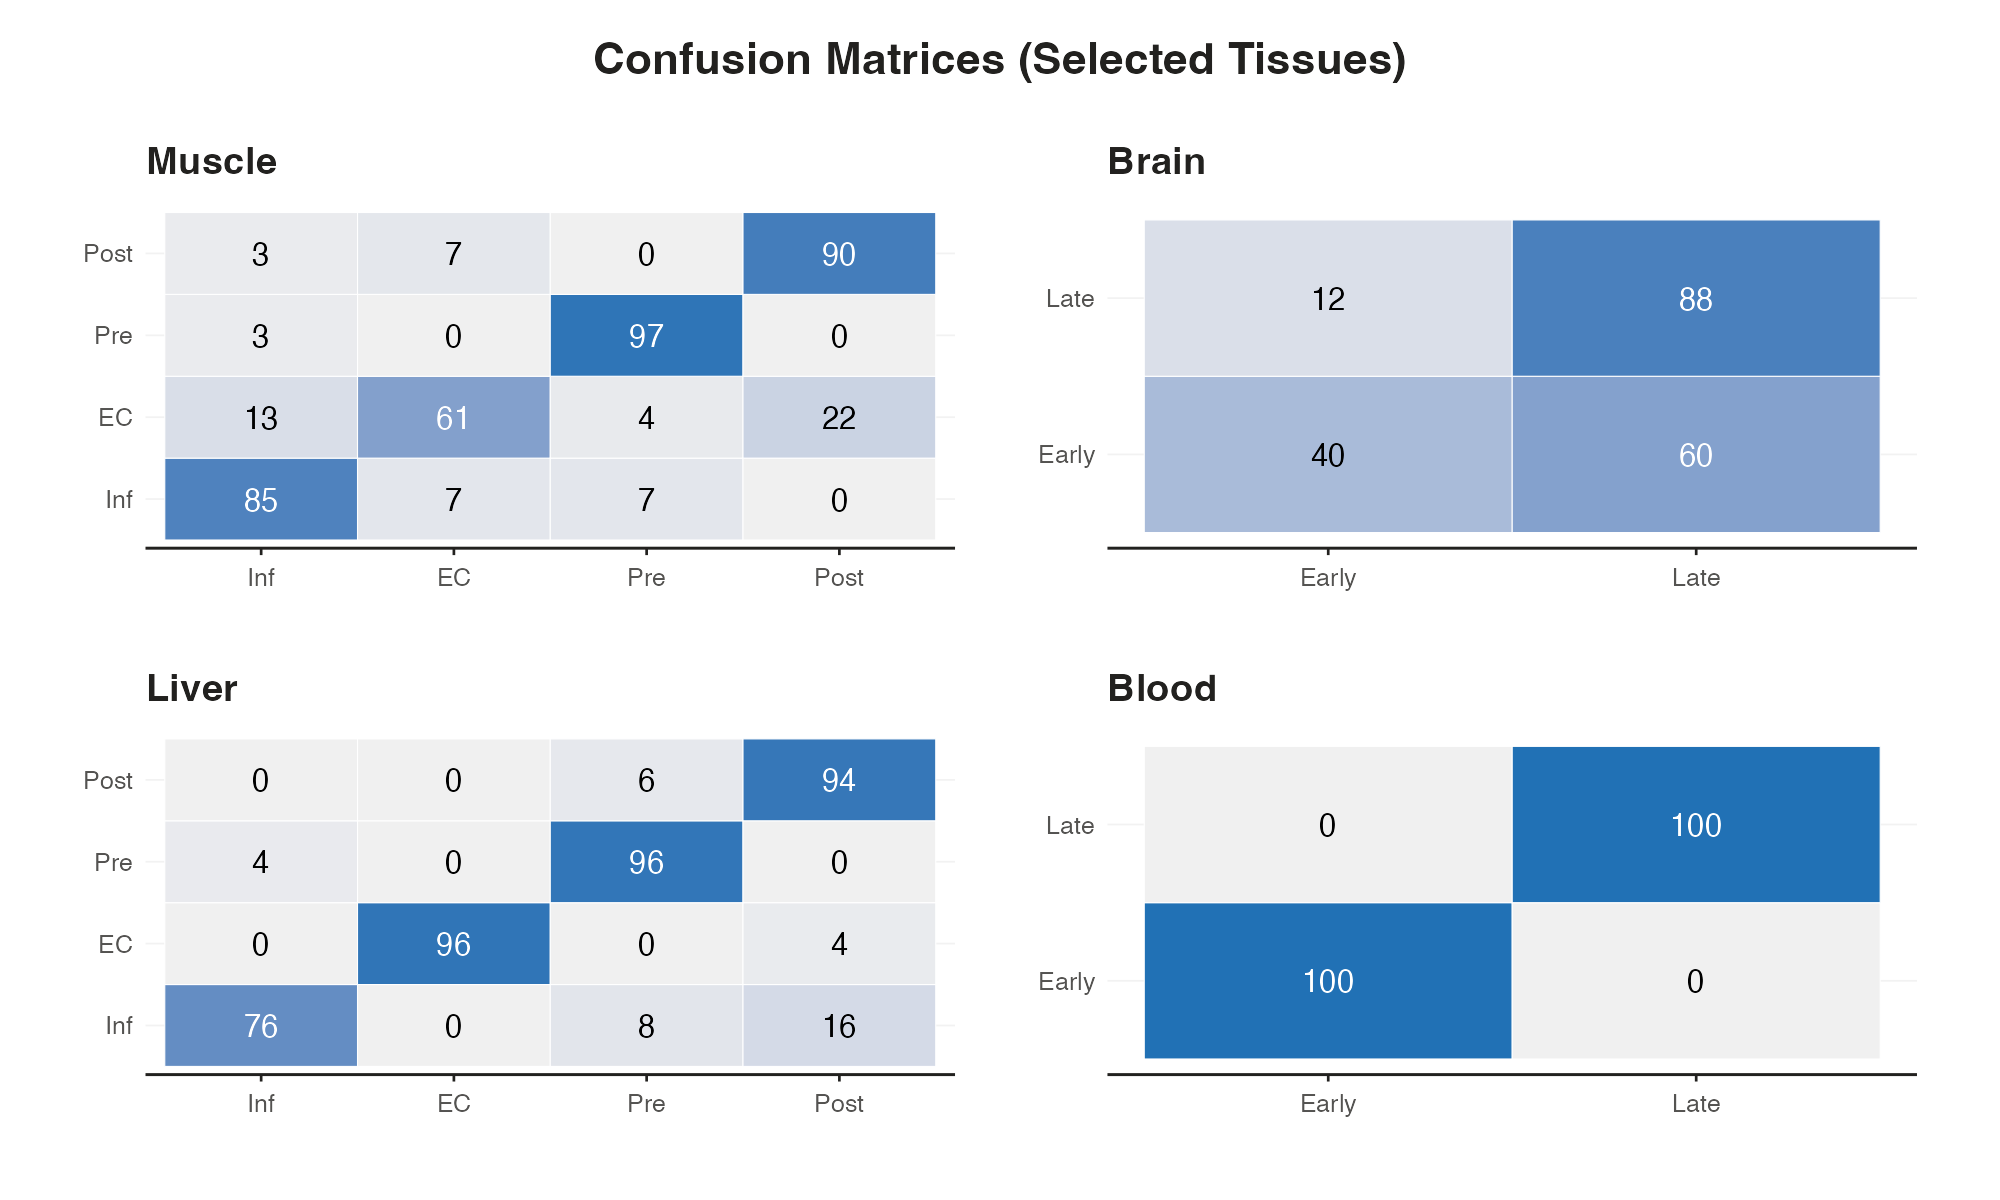
\includegraphics[width=0.85\textwidth, height=0.75\textheight, keepaspectratio]{Figures/fig2_panel_b_confusion_matrices}
    
    \vspace{0.1cm}
    \begin{center}

    \end{center}
\end{frame}

\begin{frame}{Age Correlation}
    \centering
    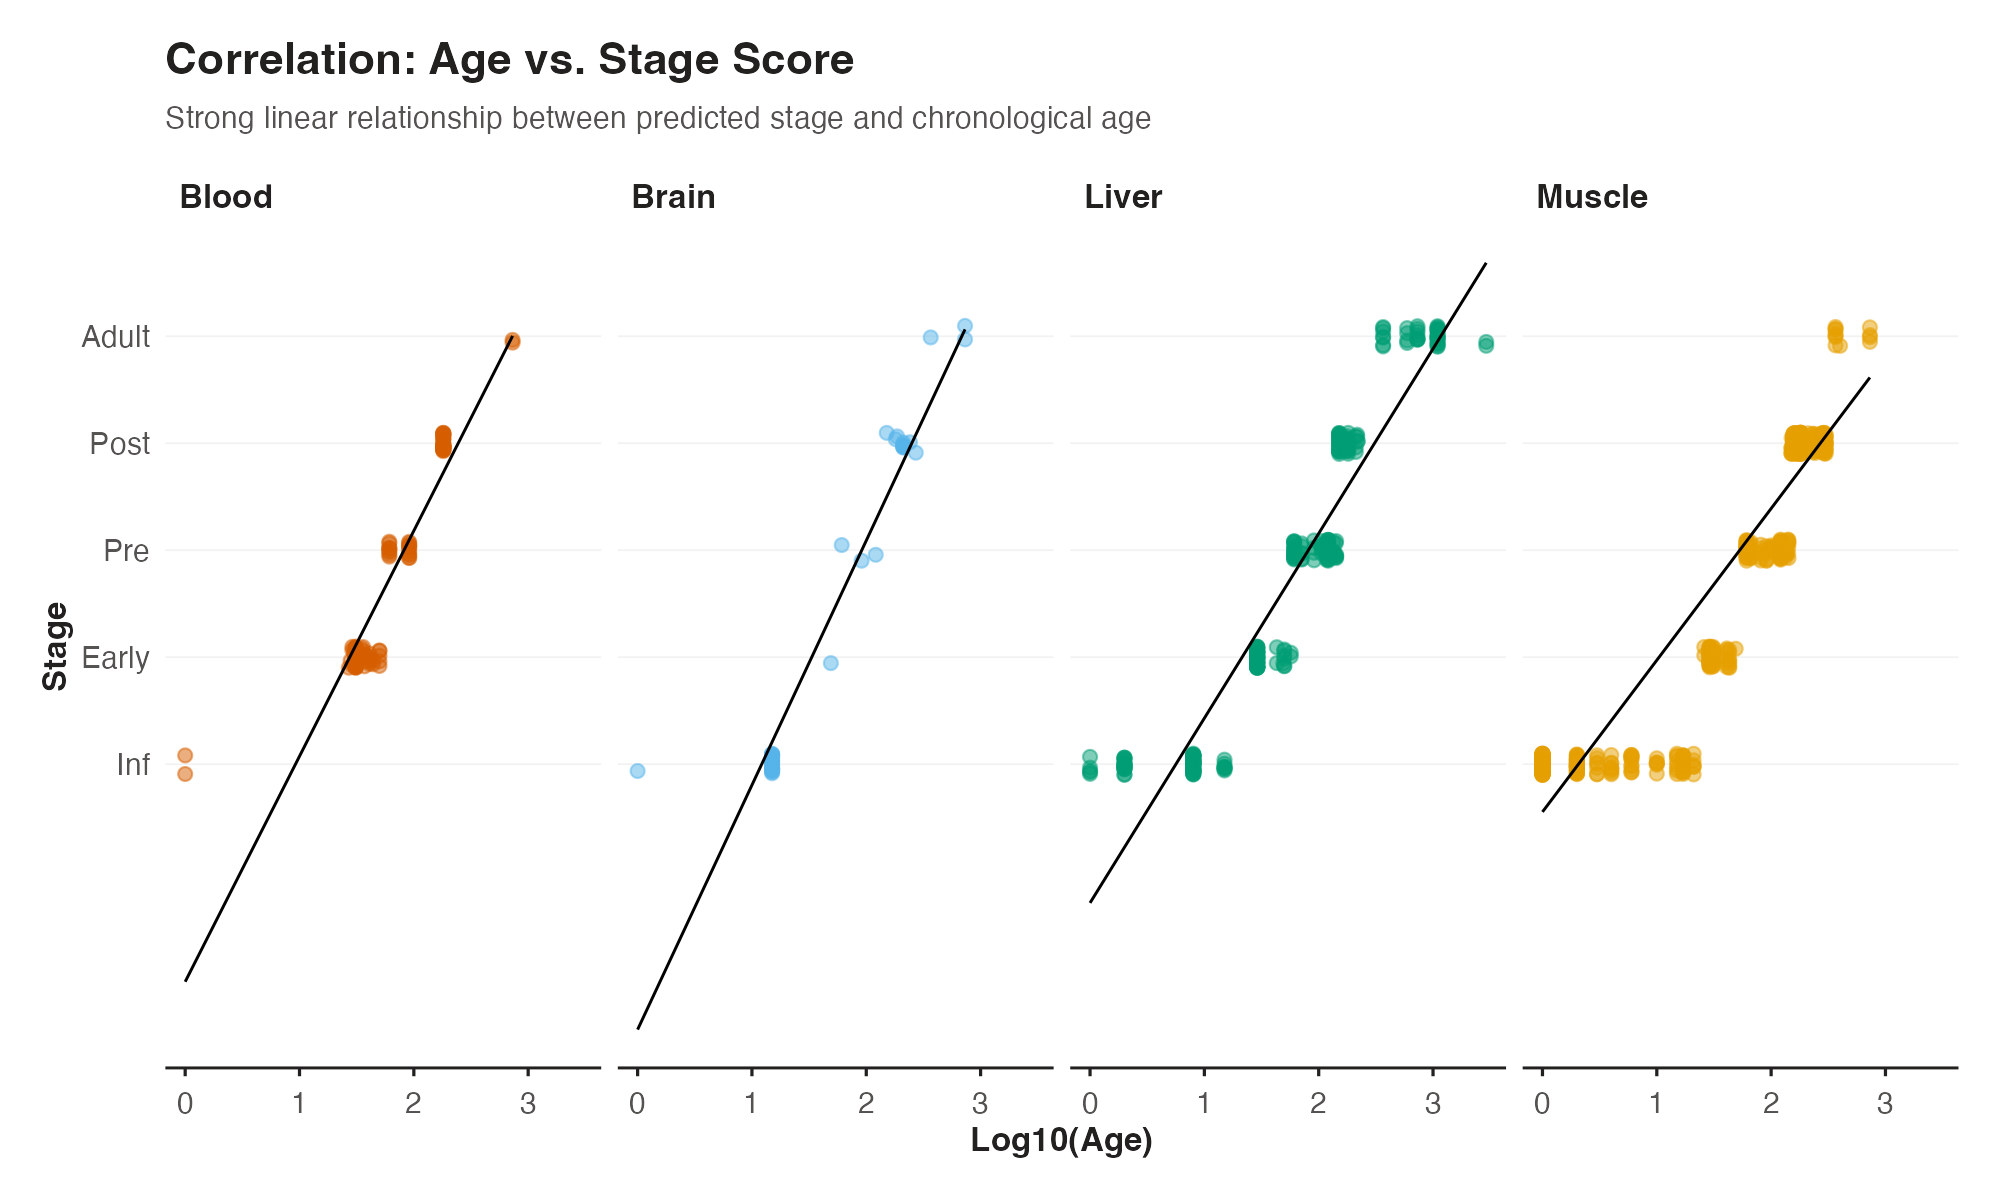
\includegraphics[width=0.85\textwidth]{Figures/fig2_panel_c_age_correlation}
\end{frame}

% ============================================================================
% SLIDE 6: Molecular Signatures
% ============================================================================
\section{Biological Insights}

% Transition slide


\begin{frame}{Feature Overlap Analysis}
    \centering
    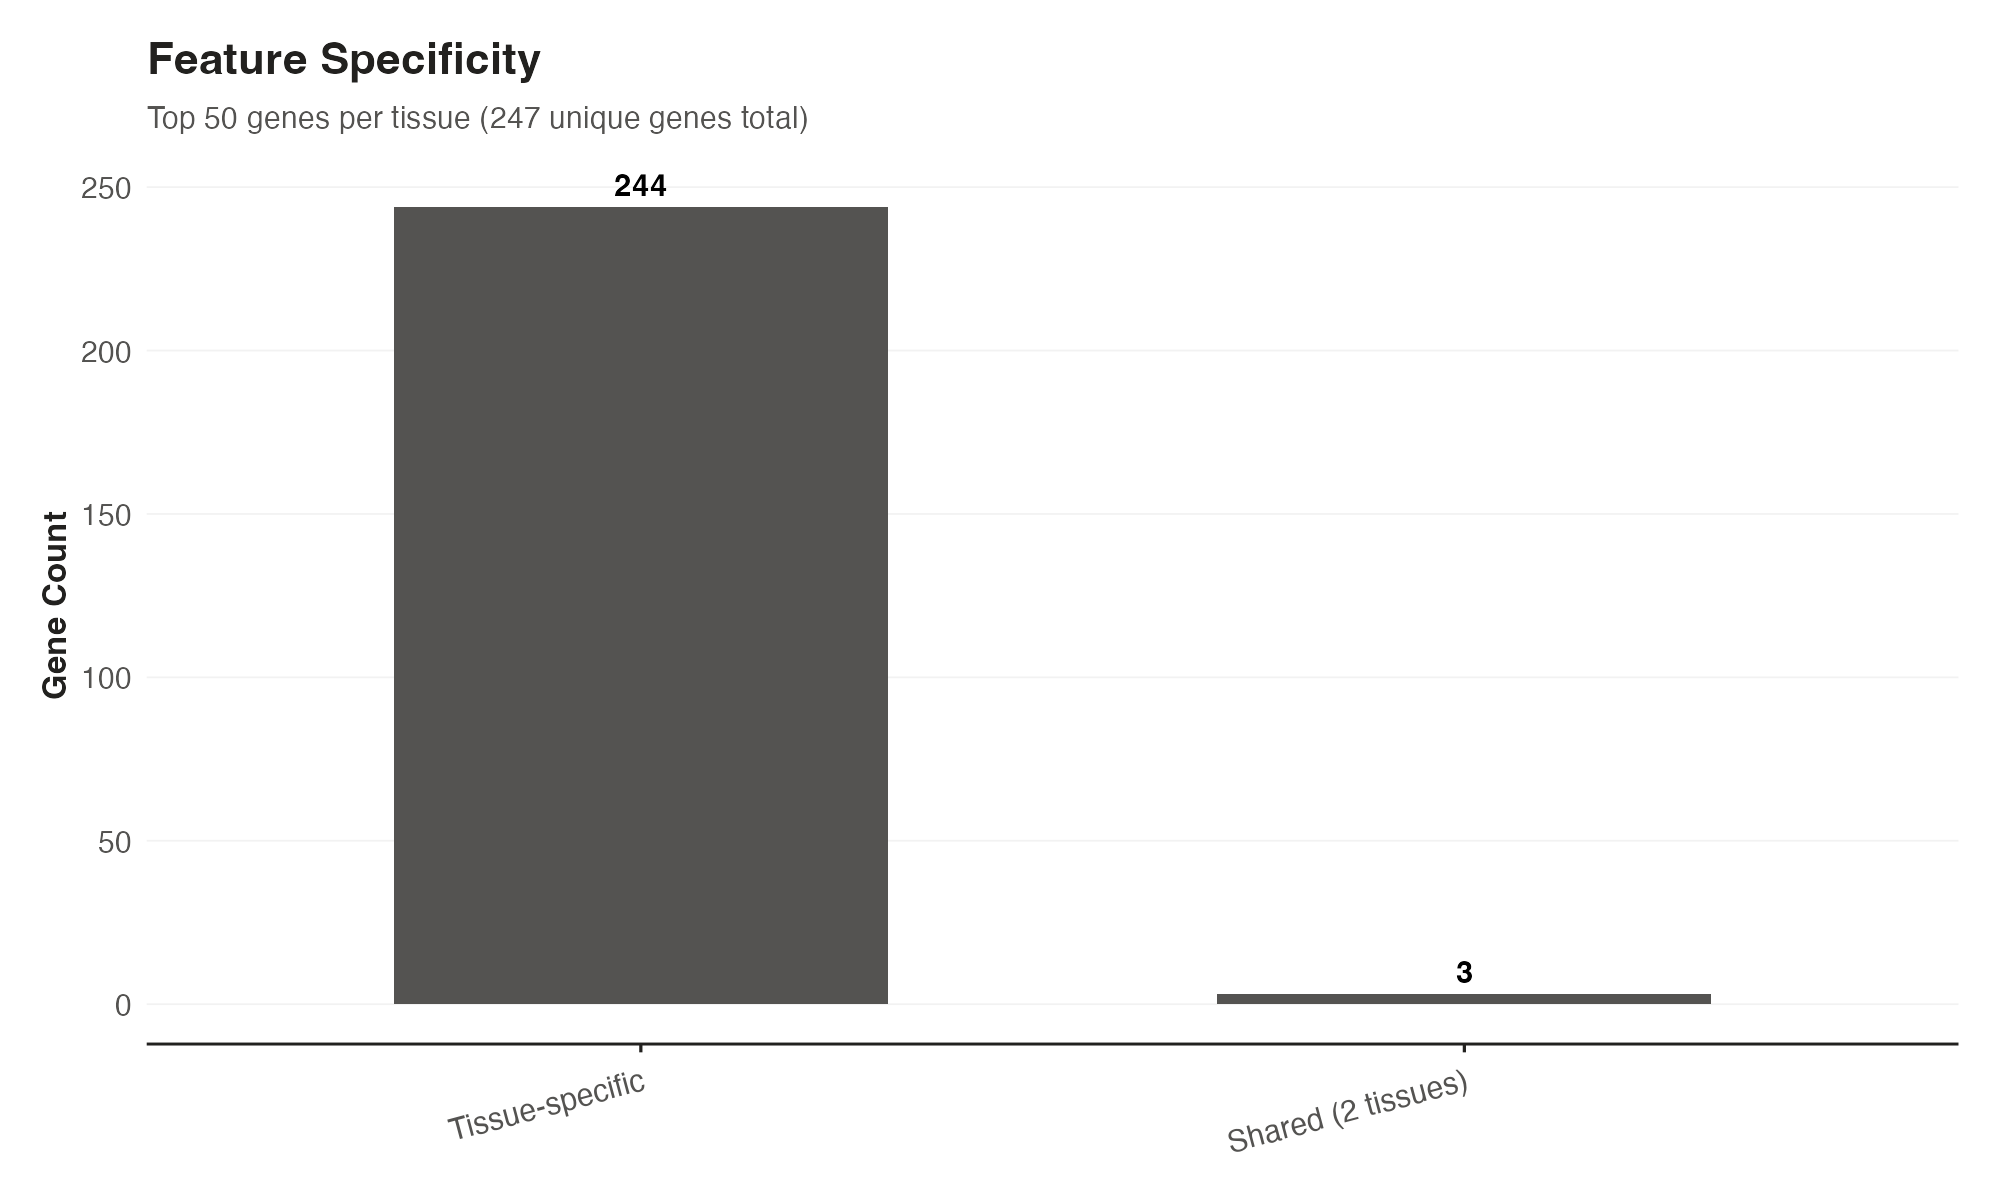
\includegraphics[width=0.85\textwidth]{Figures/fig3_panel_b_feature_overlap}
    
    \vspace{0.3cm}
    \begin{center}
        {\color{CardiffRed}\textbf{Key Finding:}} Each tissue uses distinct marker genes (Jaccard $\sim$0.3\%).\\[0.2em]
        {\color{CardiffDarkGrey}\textit{But do they converge on shared biological processes?}}
    \end{center}
\end{frame}

\begin{frame}{Tissue Specificity - UMAP}
    \centering
    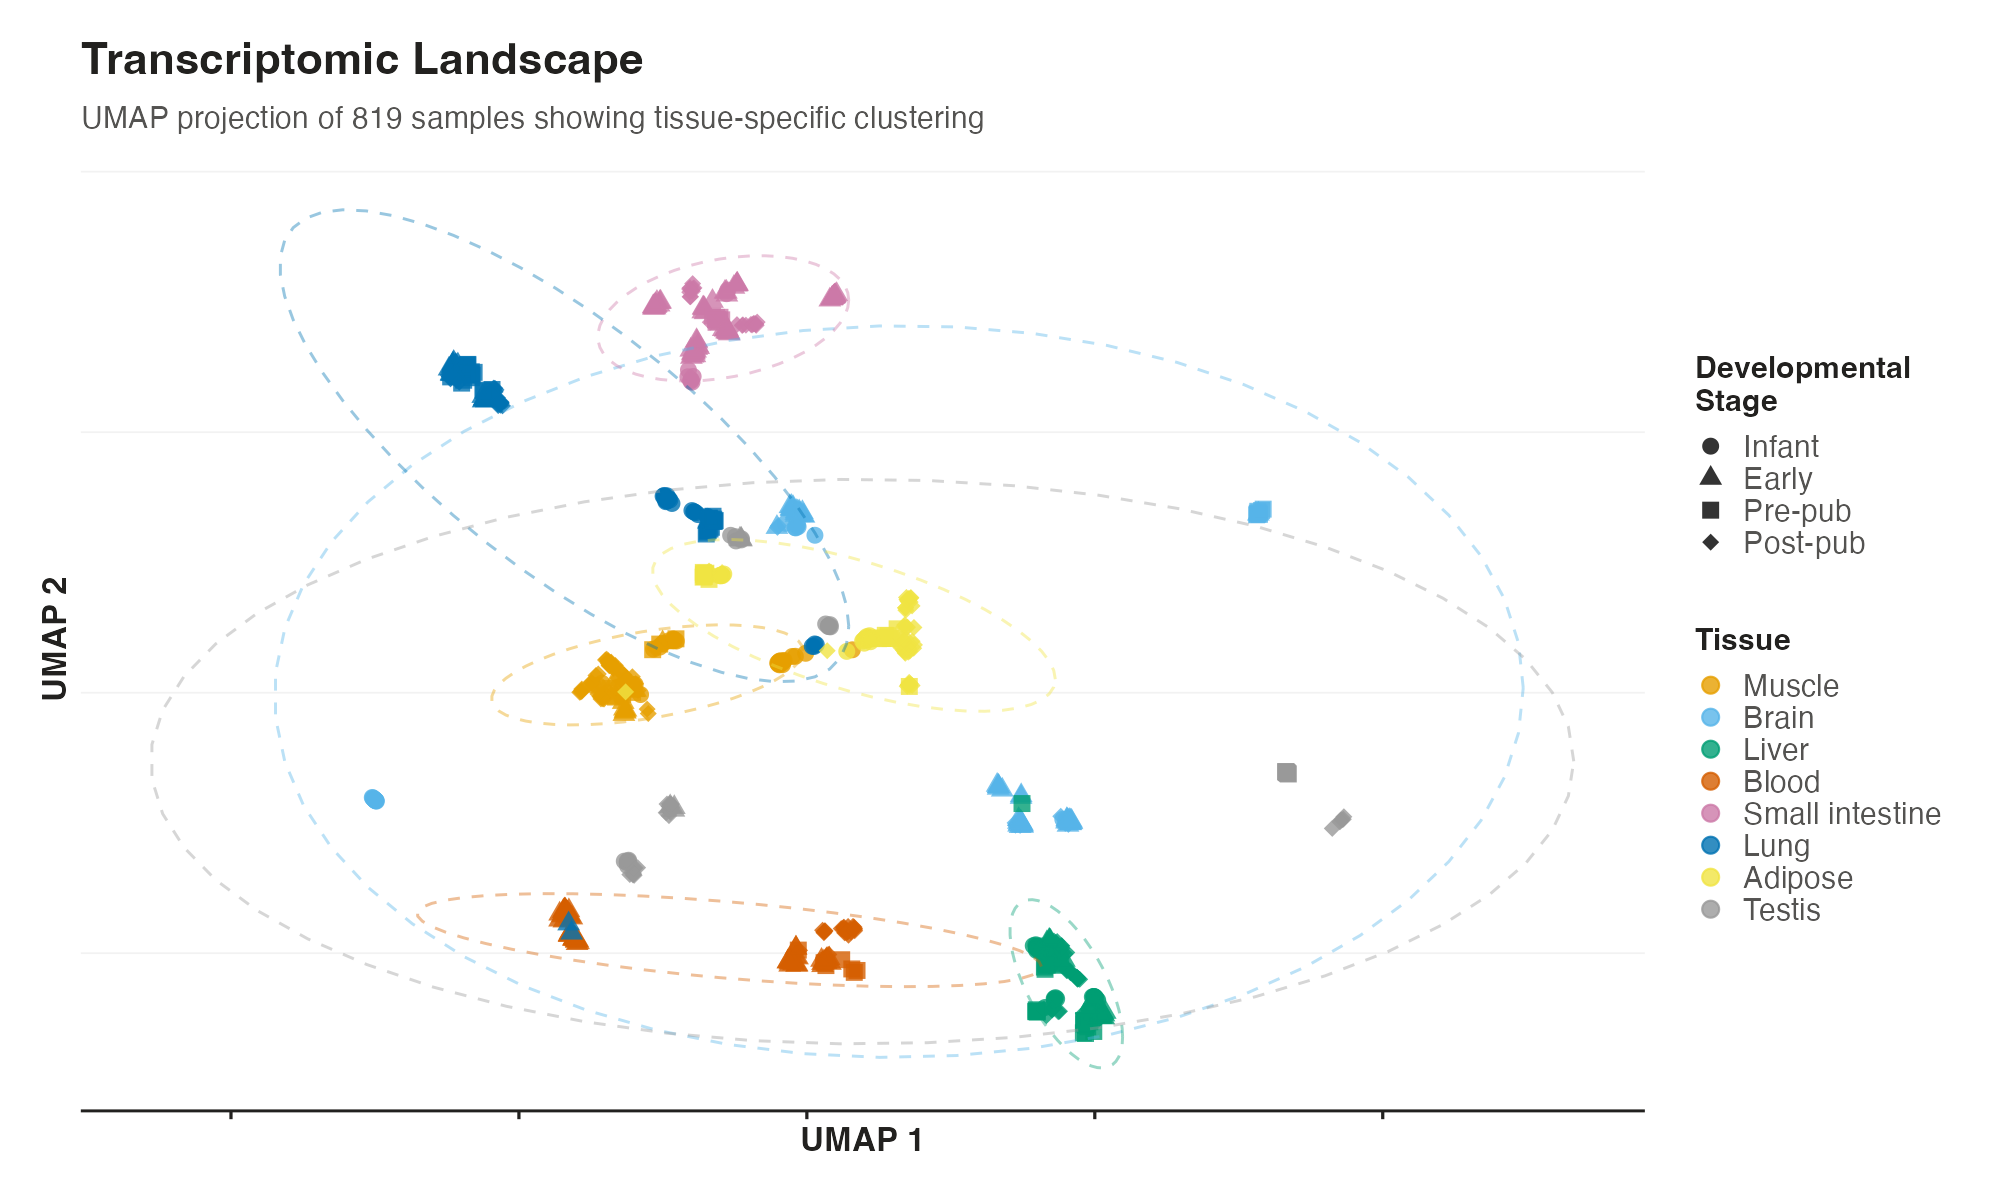
\includegraphics[width=0.85\textwidth]{Figures/fig3_panel_a_umap}
    
    \vspace{0.3cm}
    \begin{center}
        {\color{CardiffDarkGrey}Tissue-specific gene expression drives unique feature selection.}\\[0.2em]
        {\color{CardiffRed}\textit{Despite different genes, developmental trajectories may share common pathways.}}
    \end{center}
\end{frame}

\begin{frame}{Pathway Enrichment Analysis}
    \centering
    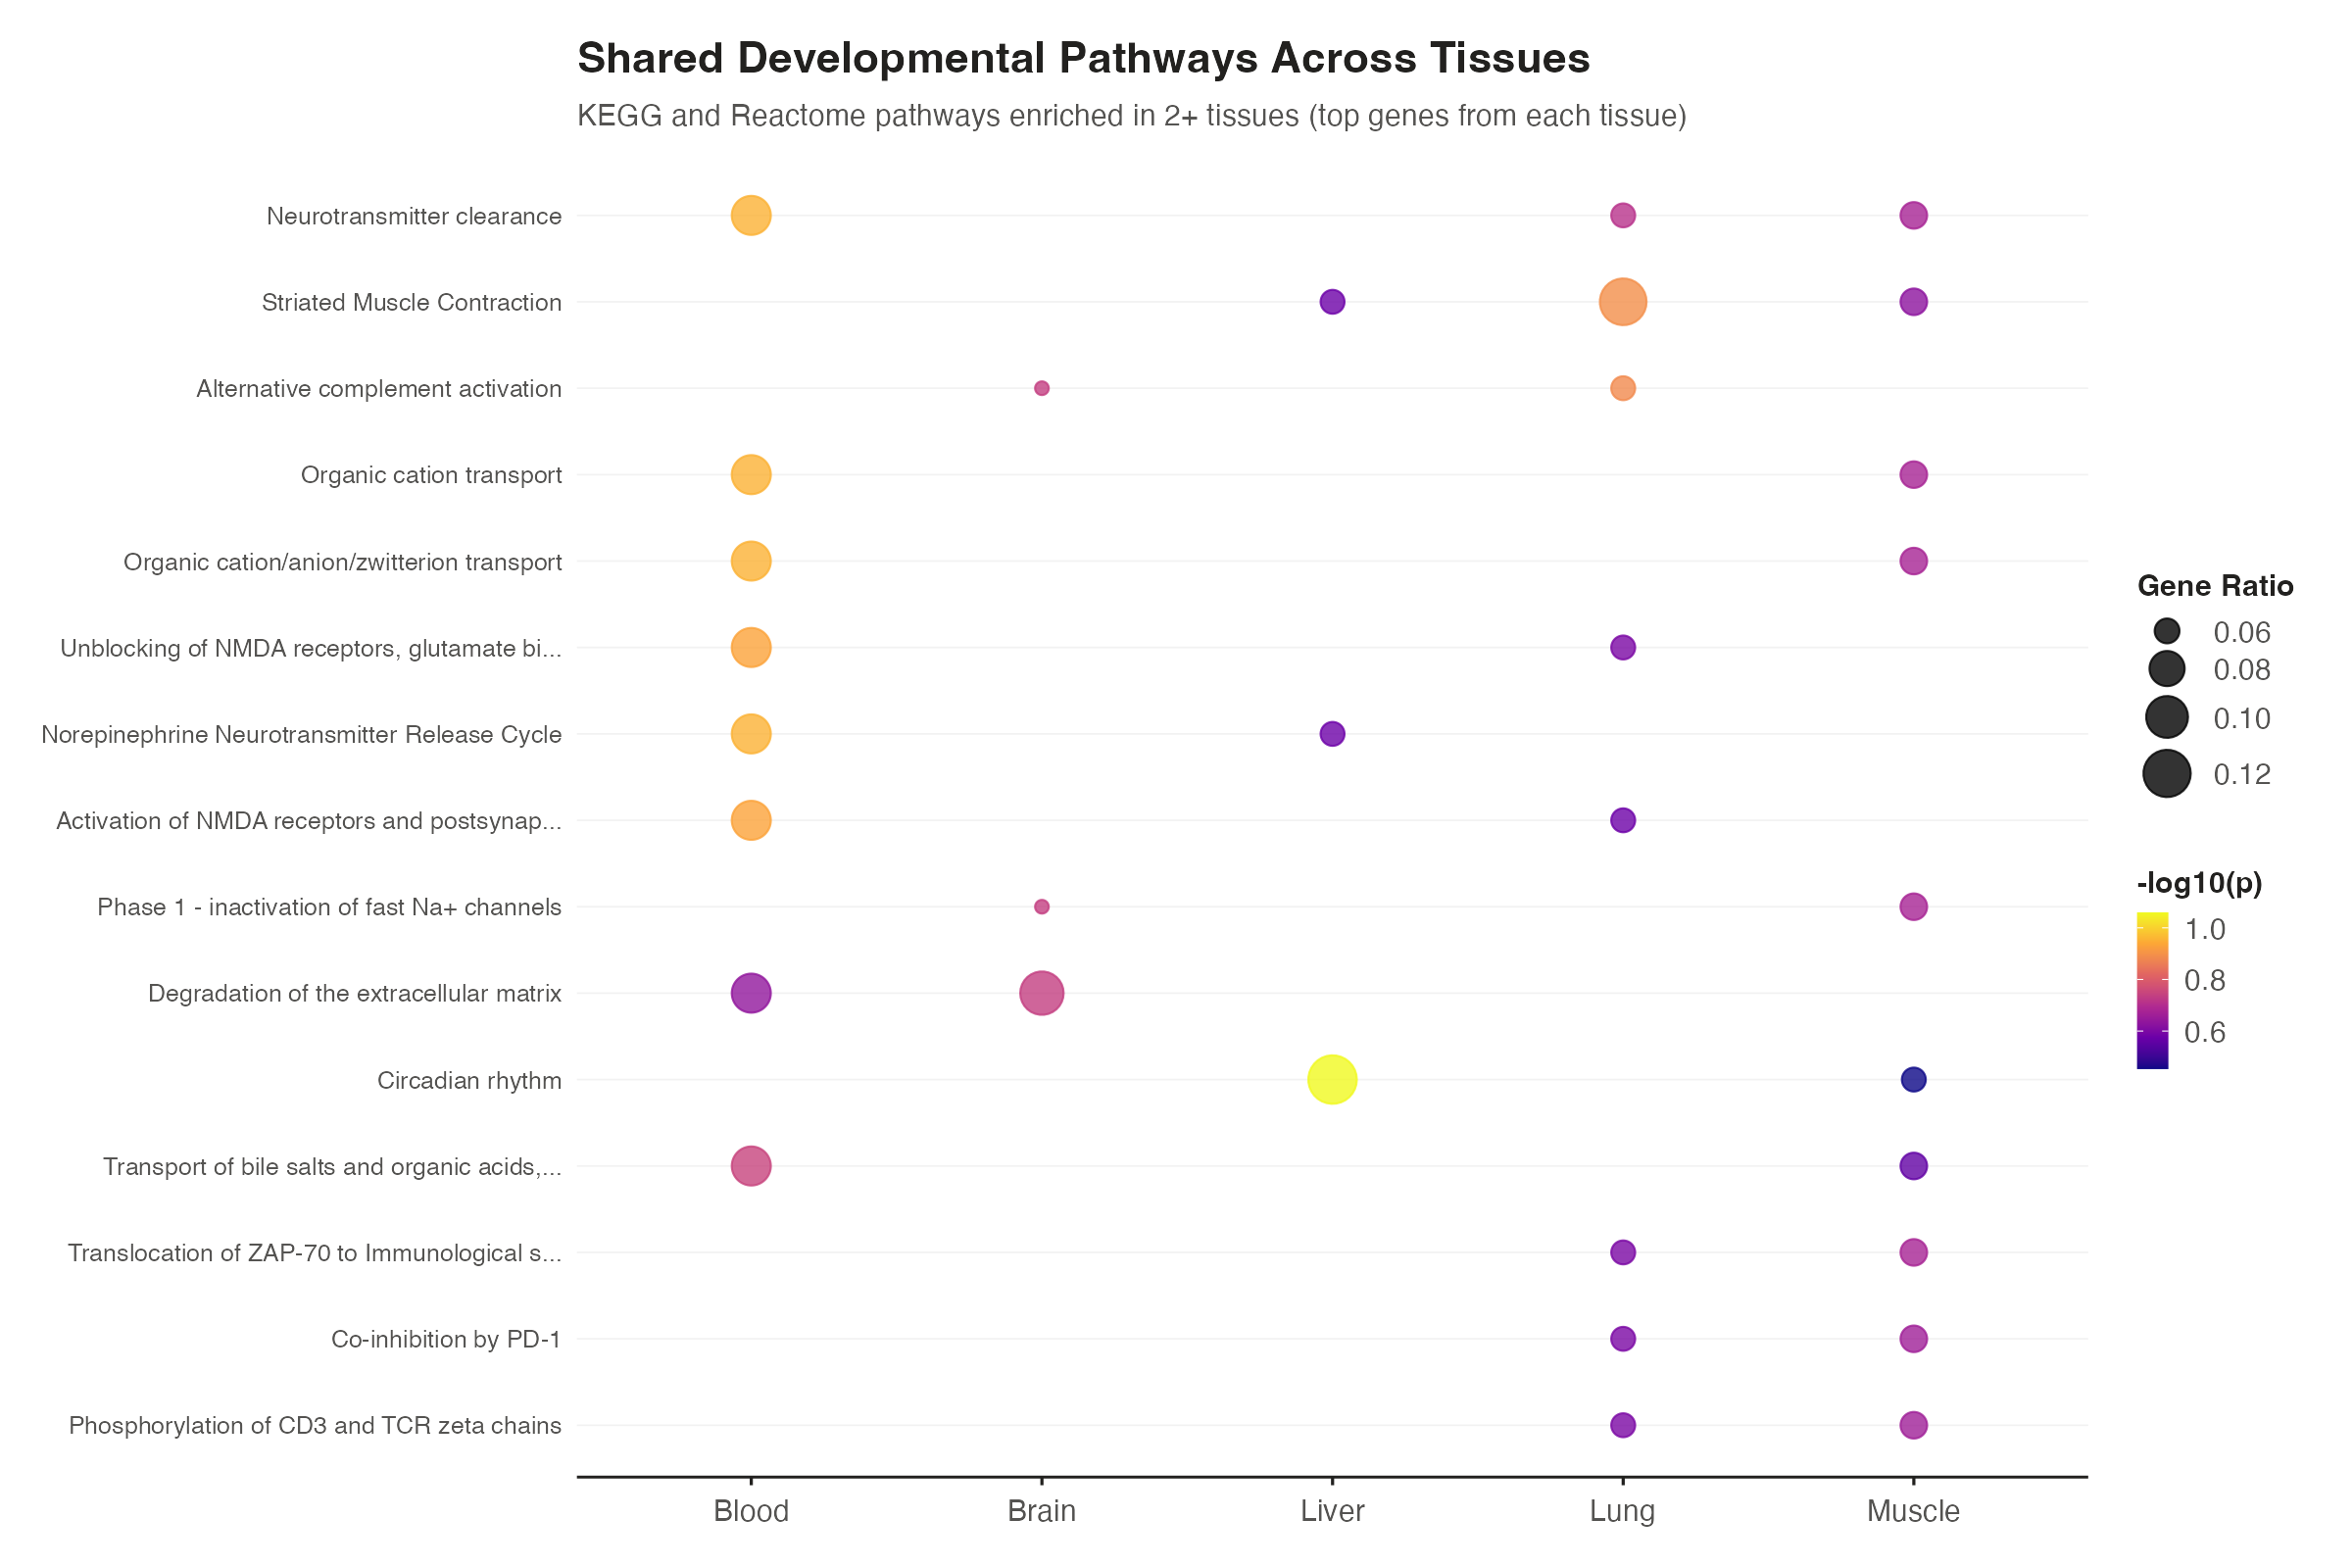
\includegraphics[width=0.85\textwidth, height=0.65\textheight, keepaspectratio]{Figures/fig5_panel_a_kegg_reactome_enrichment}
    
    \vspace{0.2cm}
    \begin{center}
        {\color{CardiffRed}\textbf{Shared Developmental Programs:}}\\[0.2em]
        {\small\color{CardiffDarkGrey}Gene regulation, metabolism, and extracellular matrix organization}
    \end{center}
\end{frame}





% ============================================================================
% SLIDE 7: Conclusion
% ============================================================================
\section{Conclusion}

\begin{frame}{Summary \& Future Directions}
    \vspace{0.3cm}
    \begin{columns}[T, onlytextwidth]
        \column{0.45\textwidth}
            \hspace{0.22cm}\cardiffHeading{Key Findings}
            \vspace{0.5em}
            \begin{itemize}
                \item Accurate staging from transcriptomics
                \item Tissue-specific molecular clocks
                \item Conserved developmental programs
            \end{itemize}
            
            \vspace{0.5em}


        \column{0.5\textwidth}
            \cardiffHeading{Next Steps}
            \vspace{0.5em}
            
            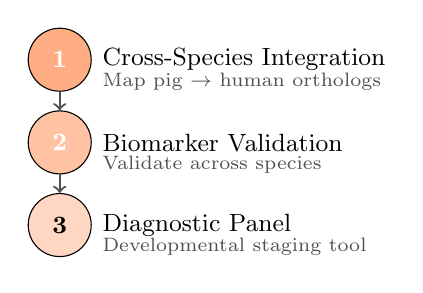
\begin{tikzpicture}[scale=0.7]
                % Step 1
                \node[draw, circle, fill=CardiffRed!80, minimum size=0.8cm, font=\bfseries\small, text=white] (s1) at (0,0) {1};
                \node[anchor=west, font=\small] at (0.6,0) {Cross-Species Integration};
                \node[anchor=west, font=\scriptsize, color=CardiffDarkGrey] at (0.6,-0.4) {Map pig $\rightarrow$ human orthologs};
                
                % Step 2
                \node[draw, circle, fill=CardiffRed!60, minimum size=0.8cm, font=\bfseries\small, text=white] (s2) at (0,-1.5) {2};
                \node[anchor=west, font=\small] at (0.6,-1.5) {Biomarker Validation};
                \node[anchor=west, font=\scriptsize, color=CardiffDarkGrey] at (0.6,-1.9) {Validate across species};
                
                % Step 3
                \node[draw, circle, fill=CardiffRed!40, minimum size=0.8cm, font=\bfseries\small] (s3) at (0,-3) {3};
                \node[anchor=west, font=\small] at (0.6,-3) {Diagnostic Panel};
                \node[anchor=west, font=\scriptsize, color=CardiffDarkGrey] at (0.6,-3.4) {Developmental staging tool};
                
                % Connecting lines
                \draw[->, thick, CardiffDarkGrey] (s1) -- (s2);
                \draw[->, thick, CardiffDarkGrey] (s2) -- (s3);
            \end{tikzpicture}
            
            \vspace{0.3em}
            {\scriptsize\color{CardiffDarkGrey}\textit{Lead: Rujing}}
    \end{columns}
\end{frame}

% ============================================================================
% SLIDE 8: End
% ============================================================================
\begin{frame}[plain]
    \begin{tikzpicture}[remember picture, overlay]
        \fill[CardiffBlack] (current page.north west) rectangle ++(\paperwidth, -\paperheight);
        \node[anchor=center] at (current page.center) {
            \fontsize{44}{52}\selectfont \color{CardiffWhite} \textbf{Thank You}
        };
        \node[anchor=south] at ([yshift=2cm]current page.south) {
            \color{CardiffGrey} \cardiffLead{liut33@cardiff.ac.uk}
        };
    \end{tikzpicture}
\end{frame}

\end{document}

